\documentclass[12pt]{report}




\usepackage[a4paper, top=25mm, bottom=25mm, left=25mm, right=25mm]{geometry}
\usepackage[inline]{enumitem}
\usepackage[linesnumbered,lined,ruled]{algorithm2e}
\usepackage[table]{xcolor}
\usepackage{
  graphicx,
  pdfpages,
  appendix,
  multicol,
  xcolor,
  soul,
  lscape,
  hyperref,
  longtable,
  listings,
  float,
  booktabs,
  setspace,
  wrapfig,
  fancyhdr
}

\pagestyle{fancy}
\fancyhf{}
\fancyhead[L]{\leftmark}
\fancyhead[R]{\thepage}

% urls + href style
\hypersetup{
  colorlinks,
  linkcolor={black},
  citecolor={blue!50!black},
  urlcolor={blue!80!black}
}

% common spacing command
\newcommand{\x}{\vspace{2mm}\\}

% highlight <colour, text>
\newcommand{\hlc}[2]{ {\sethlcolor{#1} \hl{#2}} }

\newcommand{\ra}[1]{\renewcommand{\arraystretch}{#1}}

% code styling	
\definecolor{code_comment}{rgb}{0,0.6,0}
\definecolor{code_bg}{rgb}{0.95,0.95,0.92}

\lstset{
  backgroundcolor=\color{code_bg},
  commentstyle=\color{code_comment},
  keywordstyle=\color{magenta},
  numberstyle=\tiny,
  stringstyle=\color{blue},
  basicstyle=\ttfamily\footnotesize,
  breakatwhitespace=false,
  breaklines=true,
  captionpos=b,
  keepspaces=true,
  numbers=left,
  numbersep=5pt,
  showspaces=false,
  showstringspaces=false,
  showtabs=false,
  tabsize=2,
  emphstyle={\color{orange}}
}

\setlist{nosep}


% Title page person <name, email>
\newcommand{\person}[2]{
    \vspace{0.5cm}
    \large
    \textbf{#1}\\
    #2\x
}

% Heading w/ indented content
\newcommand{\content}[2]{
    \noindent\textbf{#1}\vspace{-2mm}
    \begin{quote}
        #2
    \end{quote}
}

% persona <name, type, img, description>
\newcommand{\persona}[4]{
  \begin{center}
    \begin{tabular}[ht]{ p{0.25\textwidth} p{0.7\textwidth} }
      \multirow{3}{*}{\includegraphics[width=0.23\textwidth]{#3}} & #1 \\
      & \textit{#2}\\
      & #4
    \end{tabular}
  \end{center}
  
}

\newcommand{\tbd}{\hlc{red}{ UNFINISHED }}

\begin{document}

% BODY ONLY

\newif\ifbodyonly
\bodyonlyfalse

% 

\ifbodyonly
\else


\thispagestyle{empty}
	
\begin{center}

\vspace{0.2cm}
\Large
Electronics and Computer Science\\
Faculty of Physical Sciences and Engineering\\
University of Southampton\\
\vspace{1cm}
Thomas Smith, tcs1g20\\
\today\\
\vspace{1cm}
\textit{Using Blockchain for Video Game Distribution}\\
\vspace{1cm}
Project Supervisor: Leonardo Aniello\\
Second Examiner: tbd\\
\vspace{1cm}
A project report submitted for the award of\\
\textbf{BSc Computer Science}

\end{center}

\newpage\newpage

%% FOREWORDS

\pagenumbering{roman}
\addcontentsline{toc}{section}{Abstract}
\begin{abstract}

Video game developers will often have to rely on third party platforms for the distribution of their games; this comes at a large monetary cost to the developer and leaves users at a greater risk of censorship and with weak digital ownership that is reliant on the platform staying active. 
This project uses the Ethereum blockchain to facilitate the large-scale distribution and continuous updating of video games that allows developers to directly interact with their users, who will now have true digital ownership.

\end{abstract}\newpage
\addcontentsline{toc}{section}{Statement of Originality}
\section*{Statement of Originality}

\begin{itemize}
  \item I have read and understood the \href{}{ECS Academic Integrity}
        information and the University's \href{}{Academic Integrity
        Guidance for Students}.
  \item I am aware that failure to act in accordance with the \href{}
        {Regulations Governing Academic Integrity} may lead to the
        imposition of penalties which, for the most serious cases, may 
        include termination of programme.
  \item I consent to the University copying and distributing any or all 
        of my work in any form and using third parties (who may be based 
        outside the EU/EEA) to verify whether my work contains plagiarised 
        material, and for quality assurance purposes.
\end{itemize}
\vspace{2mm}
\noindent\textbf{\textit{You must \underline{change the statements in the boxes} if 
you do not agree with them.}}
\x
\noindent We expect you to acknowledge all sources of information (e.g. ideas, algorithms, data) using
citations. You must also put quotation marks around any sections of text that you have copied
without paraphrasing. If any figures or tables have been taken or modified from another source,
you must explain this in the caption and cite the original source.

\begin{longtable}[ht]{ | p{\textwidth} | }
  \toprule
  \textbf{ I have acknowledged all sources, and identified any content taken from elsewhere.}
  \\\bottomrule
\end{longtable}

\noindent If you have used any code (e.g. open-source code), reference designs, or similar resources that
have been produced by anyone else, you must list them in the box below. In the report, you must
explain what was used and how it relates to the work you have done.

\begin{longtable}[ht]{ | p{\textwidth} | }
  \toprule
  \textbf{I have not used any resources produced by anyone else.
  }
  \\\bottomrule
\end{longtable}

\noindent You can consult with module teaching staff/demonstrators, but you should not show anyone else
your work (this includes uploading your work to publicly-accessible repositories e.g. Github, unless
expressly permitted by the module leader), or help them to do theirs. For individual assignments,
we expect you to work on your own. For group assignments, we expect that you work only with
your allocated group. You must get permission in writing from the module teaching staff before
you seek outside assistance, e.g. a proofreading service, and declare it here.

\begin{longtable}[ht]{ | p{\textwidth} | }
  \toprule
  \textbf{I did all the work myself, or with my allocated group, and have not helped anyone else.}
  \\\bottomrule
\end{longtable}

\noindent We expect that you have not fabricated, modified or distorted any data, evidence, references,
experimental results, or other material used or presented in the report. You must clearly describe
your experiments and how the results were obtained, and include all data, source code and/or
designs (either in the report, or submitted as a separate file) so that your results could be
reproduced. 
\vspace{4mm}
\begin{longtable}[ht]{ | p{\textwidth} | }
  \toprule
  \textbf{The material in the report is genuine, and I have included all my data/code/designs. }
  \\\bottomrule
\end{longtable}

\noindent We expect that you have not previously submitted any part of this work for another assessment.
You must get permission in writing from the module teaching staff before re-using any of your
previously submitted work for this assessment.

\begin{longtable}[ht]{ | p{\textwidth} | }
  \toprule
  \textbf{I have not submitted any part of this work for another assessment.}
  \\\bottomrule
\end{longtable}

\noindent If your work involved research/studies (including surveys) on human participants, their cells or
data, or on animals, you must have been granted ethical approval before the work was carried
out, and any experiments must have followed these requirements. You must give details of this in
the report, and list the ethical approval reference number(s) in the box below.

\begin{longtable}[ht]{ | p{\textwidth} | }
  \toprule
  \textbf{My work did not involve human participants, their cells or data, or animals.}
  \\\bottomrule
\end{longtable}\newpage
\addcontentsline{toc}{section}{Acknowledgements}
\section*{Acknowledgements}

I would like to thank my supervisor, Leonardo Aniello, for his support throughout this project.\newpage

%% CONTENTS
\tableofcontents

\fi

\clearpage\pagenumbering{arabic}

%% INPUT SECTIONS


\chapter{Problem Statement}

Video games are often large and highly popular pieces of software that are typically distributed for developers by a third party platform like Steam or Epic Games. Whilst these platforms provide benefits such as availability, and some social features they have some major downsides that includes:
\vspace{1mm}
\begin{enumerate}[label=(\alph*)]
  \item taking a large cut of all revenue, \newline\textit{Steam take a 30\% cut}
  \item being vulnerable to censorship from governments, and \newline\textit{The Chinese version of Steam is heavily censored}
  \item the user's access to their games is linked to the platform. \newline\textit{If the platform shuts down, the user loses all their games}
\end{enumerate}
\vspace{1mm}
\noindent A blockchain-based platform will provide greater profits to the developer, eliminate the need for trust in a third party platform, and allow users greater control over the games they own as their access is not directly linked to one service.

\section{Goals}

The goal of this project is to implement a large-scale distribution platform that will allow game developers to release and continuously update their games on a public network by directly interacting with their users. This aims to boost revenue for the developer, reduce the risk of censorship, and improve the rights of the user in terms of digital ownership. The design should include:
\vspace{1mm}
\begin{itemize}
  \item how data is shared between nodes in the network,
  \item how downloaded data can be verified using the network,
  \item how users can be incentivised by developers to help distributed their games,
  \item how users can prove their contribution,
  \item how users can prove they have purchased a game.
\end{itemize}
\vspace{1mm}
\noindent The application will consist of a set of smart contracts, written in Solidity, as well as an interface to the blockchain written using TypeScript, with libraries such as Web3. Tools like Truffle and Ganache will also be helpful during development. 

\section{Scope}

This project will look at how the Ethereum blockchain and smart contracts can be used to create a large-scale distribution platform for video games. This be deployed to a `testnet', where Ether has no value and applications can be tested in a live environment.
\chapter{Background Research}


\section{BitTorrent}

BitTorrent~\cite{kaune_unraveling_2010,pouwelse_bittorrent_2005} is the most popular p2p file-sharing platform, in which users will barter for chunks of files by downloading and uploading them in a tit-for-tat fashion, such that peers with a high upload rate will typically also have a high download rate. For a user to download data from BitTorrent they would:

\subsection{Download Protocol}

\begin{enumerate}
  \item Find the corresponding \.torrent file that contains metadata about the torrent such as the location of a tracker, file information such as name, size and path in the directory.
  \item The user will find peers also interested in that torrent through a tracker and will establish connections with them.
  \item The data is split into constant-sized blocks and are downloaded individually. BitTorrent uses a tit-for-tat mechanism that incentivises users to contribute by providing preferable treatment to nodes who upload data as well.
  \item The user will download blocks based upon the following priority:
        \begin{enumerate}
          \item \textbf{Strict Priority} Data is split into pieces and sub-pieces with the aim that once a given sub-piece is requested then all of the other sub-pieces in the same piece are requested
          \item \textbf{Rarest First} Aims to download the piece that the fewest peers have to increase supply.
          \item \textbf{Random First Piece} When a peer has no pieces, it will try to get one as soon as possible to be able to contribute.
        \end{enumerate}
  \item The node will continuously upload blocks it has while active.
\end{enumerate}

\subsection{Availability}

It is commonly suggested that availability of torrents is the biggest issue surrounding BitTorrent as \textit{`38\% of torrents become unavailable in the first month'}~\cite{kaune_unraveling_2010} and that \textit{`the majority of users disconnect from the network within a few hours after the download has finished'}~\cite{pouwelse_bittorrent_2005}.
This paper~\cite{neglia_availability_2007} looks at how the use of multiple trackers for the same content and DHTs can be used to boost availability.



\section{Ethereum}

Ethereum is a Turing-complete, distributed, transaction-based blockchain that allows the deployment of decentralized applications through the use of smart contracts. Ether is the currency used on Ethereum and can be traded between accounts and is used to execute smart contract code on the network. 

\subsection*{Smart Contracts}

A smart contract is an executable piece of code, written in Solidity, that will automatically execute on every node in the Ethereum network when certain conditions are met. Smart contracts are enforced by the blockchain network and remove the need for intermediaries and reduce the potential of contractual disputes.
\x
Gas is used to measure the computational effort of running a smart contract and must be paid, in Ether, before being processed and added to the blockchain. This helps prevent DoS attacks and provides economic incentives for users to behave in a way that benefits the whole network.

\subsection*{Example Use Cases}

Some examples of applications that can be deployed to the Ethereum network are:

\begin{itemize}
  \item Financial applications, such as decentralised exchanges and payment systems,
  \item supply chain management and tracking,
  \item voting and governance systems,
  \item unique digital asset systems, and
  \item data storage and sharing platforms.
\end{itemize}

\chapter{Literature Review}


\section{Blockchain-Based Cloud Storage}

In table~\ref{tab:blockhain cloud storage}, I detail some examples of how blockchain has been used to solve problems within cloud storage systems. One interesting finding from these papers~\cite{sukhodolskiy_blockchain-based_2018,hasan_cloud_2019} is that blockchain can been used to provide additional services to cloud storage systems, such as monitoring access control or helping to verify the integrity of the data on these systems.

\begin{longtable}{ p{0.35\textwidth} p{0.6\textwidth} }
  \toprule
  \textbf{Paper} & \textbf{Description of Solution}
  \\\midrule\midrule
  Blockchain Based Data Integrity Verification in P2P Cloud Storage~\cite{yue_blockchain_2018}
  & This paper uses Merkle trees to help verify the integrity of data within a P2P blockchain cloud storage network as well as looking at how different structures of Merkle trees effect the performance of the system.
  %
  \x
  Deduplication with Blockchain for Secure Cloud Storage~\cite{li_deduplication_2018}
  & This paper describes a deduplication scheme that uses the blockchain to record storage information and distribute files to multiple servers. This is implemented as a set of smart contracts.
  %
  \x
  Block-secure: Blockchain based scheme for secure P2P cloud storage~\cite{li_block-secure_2018}
  & A distributed cloud system in which users divide their own data into encrypted chunks and upload those chunks randomly into the blockchain, P2P network. 
  %
  \x
  Blockchain-Based Medical Records Secure Storage and Medical Service Framework~\cite{chen_blockchain-based_2018}
  & Describes a secure and immutable storage scheme to manage personal medical records as well as a service framework to allow for the sharing of these records.
  %
  \x
  A Blockchain-Based Access Control System for Cloud Storage~\cite{sukhodolskiy_blockchain-based_2018}
  & This paper describes a method for using blockchain to facilitate the access control over a cloud storage system. The blockchain stores an immutable record of all `\textit{meaningful security events}', such as key generation, access policy, assignment, etc.
  %
  \x
  Cloud Data Provenance using IPFS and Blockchain Technology~\cite{hasan_cloud_2019}
  & Uses blockchain technology and IPFS to provide an efficient way to securely store provenance~\footnote{Provenance data are access logs of stored data that can trace the integrity of data and will contain private user information.} data such that it is out of reach of adversaries, but can be used to verify the integrity of data on a cloud storage system. 
  \\\bottomrule\bottomrule
  \caption{\textit{Examples of blockchain cloud storage systems~\cite{sharma_blockchain_2021} }}
  \label{tab:blockhain cloud storage}
\end{longtable}



\chapter{Design}


\section{Stakeholders \& Requirements}


\subsection{Stakeholders}

\newcommand{\primary}{\hlc{cyan}{ PRIMARY }\\}
\newcommand{\secondary}{\hlc{yellow}{ SECONDARY }\\}
\newcommand{\tertiary}{\hlc{green}{ TERTIARY }\\}

\paragraph{Game Developers}\primary
This group will use the application to release their games and its updates to their users, who they will reward for helping to distribute it.

\paragraph{Players}\primary
This group will use this application to downloaded and update their games off of. They may also contribute to the distribution of the games to other players for an incentive provided by the developers.

\paragraph{Game Distribution Platforms}\secondary
This group consists of platforms like Steam or Epic Games, which serve as the main competitor to this application. It is likely that as more developers choose this application, this group will see a loss in revenue. 

\paragraph{}\tertiary

\subsection{Requirements}

Tables~\ref{tab:functional-requirements} and~\ref{tab:non-functional-requirements} show the functional and non-functional requirements of this project organized using MoSCoW prioritisation. 

\subsubsection*{Functional Requirements}

\begin{longtable}{ p{.1\textwidth} p{.8\textwidth} }
  \toprule
  \textbf{ID} & \textbf{Description}
  \\\midrule\midrule
  \multicolumn{2}{c}{\cellcolor{red!70}\textit{Must}}\\\midrule
  F\_M1 & Store software metadata on a blockchain\\
  F\_M2 & A node must request individual shards from its peers\\
  F\_M3 & A node must be able to discover peers relevant to the software it wants\\
  F\_M4 & Software must be updatable through the blockchain\\
  F\_M5 & A node must be able to upload software\\
  F\_M6 & A node must be able to download software in its entirety from nodes in the same network.\\
  F\_M7 & A node must be able to verify the integrity of each block it downloads\\
  F\_M8 & The application should run on the Ethereum network\\
  F\_M9 & Users must be able to purchase games from developers over the network\\
  F\_M10 & Users must be able to prove they have purchased a game\\
  \midrule\multicolumn{2}{c}{\cellcolor{orange!70}\textit{Should}}\\\midrule
  F\_S1 & Seeders should have a way to prove how much data they have seeded\\
  F\_S2 & Seeders will only upload content to users who have a valid proof of purchase\\
  \midrule\multicolumn{2}{c}{\cellcolor{green}\textit{Could}}\\\midrule
  F\_C1 & Allow users to request specific software versions\\
  \midrule
  \bottomrule
  \label{tab:functional-requirements}
\end{longtable}

\subsubsection*{Non-Functional Requirements}

\begin{longtable}{ p{.1\textwidth} p{.8\textwidth} }
  \toprule
  \textbf{ID} & \textbf{Description}
  \\\midrule\midrule
  \multicolumn{2}{c}{\cellcolor{red!70}\textit{Must}}\\\midrule
  NF\_M1 & The application is decentralized and cannot be controlled by any one party\\
  NF\_M2 & Any user must be able to join and contribute to the network\\
  NF\_M3 & Game uploaders should be publicly identifiable\\
  NF\_M4 & Metadata required to download the game should be immutable\\
  \midrule\multicolumn{2}{c}{\cellcolor{orange!70}\textit{Should}}\\\midrule
  NF\_S1 & This application must be scalable, such that many users can upload and download the same game at the same time.\\
  NF\_S2 & Only the original uploader can upload an update to their game\\
  \midrule\multicolumn{2}{c}{\cellcolor{green}\textit{Could}}\\\midrule
  \\
  \midrule
  \bottomrule
  \label{tab:non-functional-requirements}
\end{longtable}

\section{Design Considerations}

\subsection*{Type of Blockchain}

To satisfy \textbf{NF\_M2} and \textbf{NF\_M1}, we will need to use a public blockchain, which will benefit our project by:

\begin{itemize}
  \item being accessible by a greater amount of people, which should boost availability and scalability (satisfying \textbf{NF\_S1}),
  \item reducing the risk of censorship,
  \item providing greater data integrity (\textbf{NF\_M4})
\end{itemize}

\noindent Ethereum is a public blockchain that allows developers to publish their own distributed applications to it; it comes with an extensive development toolchain so is an obvious choice for this project (\textbf{F\_M8}).


\subsection*{Uploading Content}
\label{subsec:upload-content}

For developers to upload their game (\textbf{F\_M5}), they must provide a digital certificate to prove their identity (\textbf{NF\_M3}) as well as the required metadata (\textbf{F\_M1}) for identifying\footnote{Such as the name, release date, version number, creator and price.}, downloading\footnote{Such as the address of where to purchase the game, the digital certificate of who you're purchasing off and a tracker} and verifying the game\footnote{The root hash and the hashes of each block of data}. The developer is then expected to allow users to purchase the game off them and seed the game to at least an initial group of users.

\begin{figure}[ht]
  \centering
  \includegraphics[width=.85\textwidth]{images/diagrams/block-body.png}
  \caption{\textit{How shard data is stored.}}
  \label{fig:hash-storage}
\end{figure}

\subsection*{Purchasing Content}

Users will purchase content from developers using Ether (\textbf{F\_M9}) and will be provided with a proof of purchase (\textbf{F\_M10}) that is encrypted with their private key and can be used by any node in the network to verify the purchase.

\subsection*{Downloading Content}

Games will be content addressable, using their root hash stored on the blockchain, and will allow users to discover nodes to download off of (\textbf{F\_M3}). Once a user finds a node it will:

\begin{enumerate}
  \item Send their proof of purchase of the desired game (\textbf{F\_S2}).
  \item request individual shards from the node using the shard's hash (\textbf{F\_M2}),
  \item use the metadata from the blockchain to verify the block's contents (\textbf{F\_M7}),
  \item send a confirmation message that proves the successful transfer of a block (\textbf{F\_S1}), 
  \item and repeat this until the entirety of the game is installed (\textbf{F\_M6}).
\end{enumerate}

\noindent Shards will be downloaded in a similar order to that of BitTorrent, which is described in Section~\ref{subsec:bittorrent-download}.

\subsection*{Updating Content}

To satisfy \textbf{F\_M4}, developers will perform the same steps as in Section~\ref{subsec:upload-content} but will also include the hash of a previous block that contains the older version of the game. This will include the restriction that only the original uploader can upload an update to a piece of software (\textbf{NF\_S2}).

\begin{figure}[ht]
  \centering
  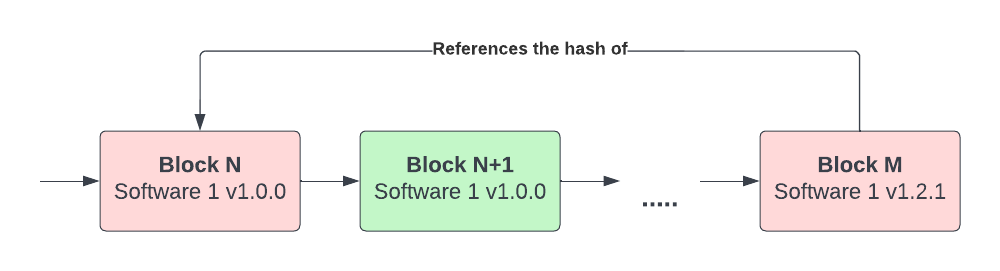
\includegraphics[width=.85\textwidth]{images/diagrams/update-software.png}
  \caption{\textit{How blocks can relate to older blocks.}}
\end{figure}

\noindent It is likely that many shards will persist between versions so a node will only ever download the changed or new data. To satisfy \textbf{F\_C1}, a node may optionally keep older shards that have been removed or changed.


\subsection*{Proving Contribution}

When a user purchases a piece of software they will be granted a unique seeder token. When a user successfully downloads a shard of data off of a peer they will reply with a confirmation message, containing this seeder token, that is encrypted using the developers public key. When a user wants to prove that they have contributed to the distribution of the game, they will send a collection of these messages to the developer, who will judge their validity.

\subsection*{Sequence Diagram}

\begin{figure}[ht]
  \centering
  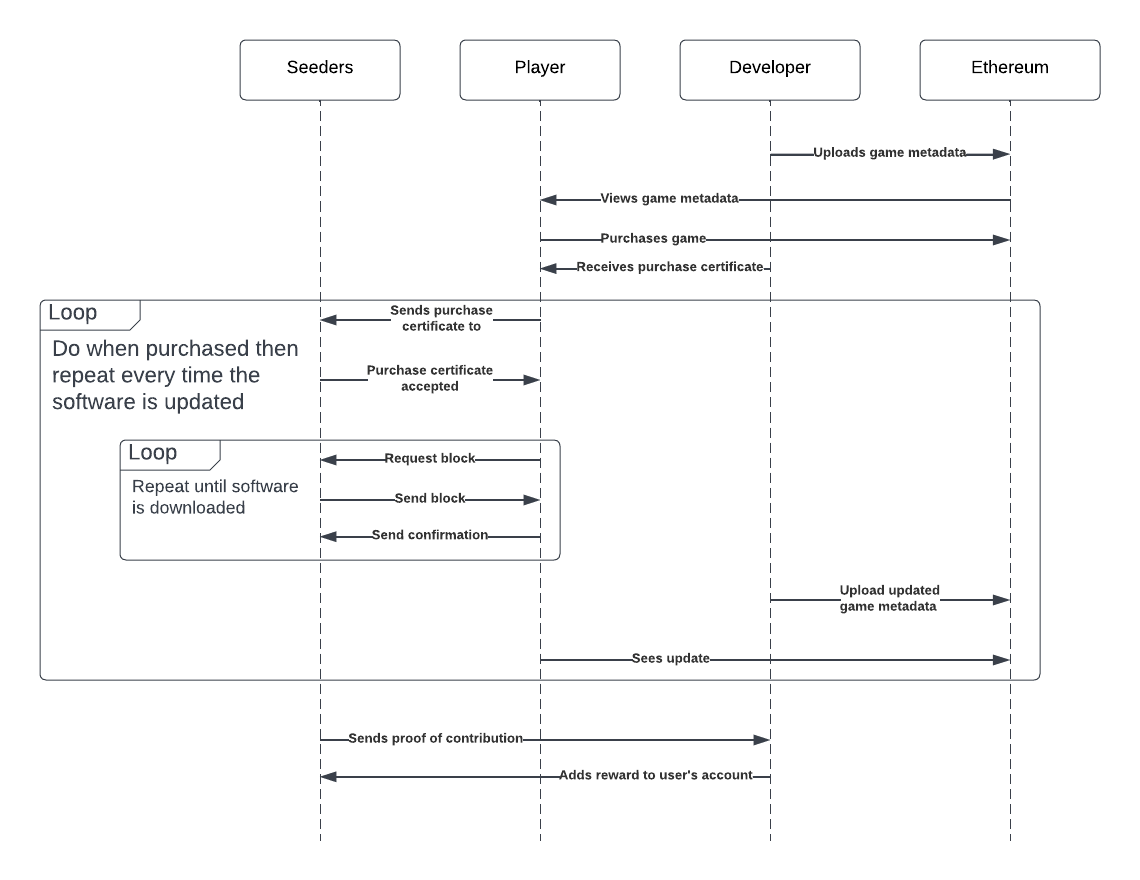
\includegraphics[width=.95\textwidth]{images/diagrams/seqeunce-diagram.png}
  \caption{\textit{The main interactions within the application.}}
\end{figure}

\section{Backend}

The backend code for this application was written based upon the design from Section~\ref{subsec:backend} and was done using the following tools:

\begin{longtable}{p{0.15\textwidth} p{0.7\textwidth}}
  \toprule
  \textbf{Tool} & \textbf{Description \& Reasoning}
  \\\midrule\midrule
  Go~\cite{noauthor_go_nodate}
  & Go was chosen because of its simple syntax, high performance, strong standard library and third party packages for interacting with Ethereum.
  \\
  go-ipfs-api~\cite{noauthor_go-ipfs-api_2023}
  & A Go package used for interacting with the Kubo implementation of IPFS that gave an easy interface for downloading and uploading data to Kubo.\\
  go-ethereum~\cite{noauthor_go-ethereum_nodate}
  & A collection of tools used for interacting with Ethereum including an Ethereum CLI client Geth, and a tool for converting Ethereum contracts into Go packages.\\
  Zap~\cite{noauthor_zap_2023}
  & A logging library that is much faster than the standard library implementation and has better customisation. \\
  Viper~\cite{noauthor_viper_nodate}
  & A configuration file management library that helps read, write, and access configuration options written to file.
  \\\bottomrule\bottomrule
  \caption{The tools used to develop the backend}
\end{longtable}

\section{Smart Contract}

To write and deploy a smart contract that met the criteria specified in Section~\ref{subsec:design-con-eth}, I used the following tools:

\begin{longtable}{p{0.15\textwidth} p{0.7\textwidth}}
  \toprule
  \textbf{Tool} & \textbf{Description \& Reasoning}
  \\\midrule\midrule
  Solidity~\cite{noauthor_solidity_nodate}
  & The language used to write smart contracts for the Ethereum blockchain.\\
  Sepolia~\cite{noauthor_sepolia_nodate}
  & An Ethereum test-net that used to deploy my smart contract to. One of the main benefits was that it provides a fast transaction time for quick feedback.\\
  Alchemy~\cite{noauthor_alchemy_nodate}
  & Alchemy provides useful tools for interacting with Ethereum and specifically Sepolia, such as an ETH faucet and an RPC URL.\\
  MetaMask~\cite{noauthor_crypto_nodate}
  & A browser-based wallet that can easily be conencted to other tools such as Alchemy or Remix.\\
  Remix~\cite{noauthor_remix_nodate}
  & A browser-based IDE for writing smart contracts that allows for easy deployment.
  \\\bottomrule\bottomrule
  \caption{The tools used for deployment of my smart contract}
\end{longtable}

\vspace{2mm}\noindent
The contract was successfully deployed~\cite{etherscanio_deployed_nodate} to the Sepolia test-net and can be interacted with by any user.

\section{Frontend}

\begin{longtable}{p{0.15\textwidth} p{0.7\textwidth}}
  \toprule
  \textbf{Tool} & \textbf{Description \& Reasoning}
  \\\midrule\midrule
  Wails~\cite{noauthor_wails_nodate}
  & Allows you to add a webkit frontend to a Go application, so that you can use a modern web framework. This allowed me to easily create a reactive UI using tools I was previously familiar with.

  Wails allows you to implement a controller using functions written in that can be called from the frontend and can emit events that trigger actions in the frontend.
  \\
  Vue.js v3~\cite{noauthor_vuejs_nodate}
  & A reactive, component based web-framework that allows me to create reusable components that react to changes in state and can trigger events at different points in a components lifecycle.
  
  The Vue Router~\cite{noauthor_vue_nodate} package was used to add multiple pages to the application and markdown-it~\cite{noauthor_markdown-it_2023} was used to render markdown files.
  \\
  Pinia~\cite{noauthor_pinia_nodate}
  & A state management tool for Vue.js that boosts the reusabiltiy of components and reduces the overall complexity of the frontend. 
  \\
  SASS~\cite{noauthor_sass_nodate}
  & An extension of CSS that is used to style DOM elements. This was essential in making the UI look nice and be accessible.
  \\
  \bottomrule\bottomrule
\end{longtable}

\section{Other Tools}

The following tools were also used throughout development:

\begin{longtable}{p{0.15\textwidth} p{0.7\textwidth}}
  \toprule
  \textbf{Tool} & \textbf{Description \& Reasoning}
  \\\midrule\midrule
  Git~\cite{noauthor_git_nodate}\newline GitHub~\cite{noauthor_github_nodate}
  & A version control system used in conjunction with GitHub. Creating periodic commits meant I always had a recent backup available and could easily backtrack to help find issues.
  Use of a GitHub Actions helped remind me that not all of my tests passed at all times :(.\\
  LaTeX~\cite{noauthor_latex_nodate}
  & Used for the write-up of this document. LaTeX was useful in creating a large document and has many packages that help with referencing and design.\\
  VSCode~\cite{noauthor_visual_nodate}
  & My code editor of choice for this project as it allowed me to seamlessly work on both my frontend and backend code at once.\\
  Lucidchart~\cite{noauthor_lucidchart_nodate}
  & Lucidchart was used to create all of the diagrams for this project.
  \\\bottomrule\bottomrule
  \caption{General purpose tools used for this project}
\end{longtable}


\section{Justification of Approach}

\section{Limitations}

This project will not attempt to mimic any of the social features (friends, achievements, message boards, etc.) provided by platforms like Steam.
\x
Section~\ref{subsec:availability} highlights the issue of availability in p2p sharing networks and this platform will likely suffer from similar issues. These can be mitigated by having an active community or good incentives to help distribute the game.
\chapter{Implementation}


\section{Components}

The diagram in Figure~\ref{fig:impl-layers} shows the main components of the application and their relationships. The following sections will discuss these in detail and provide a justification as to their existence.

\begin{figure}[ht]
  \centering
  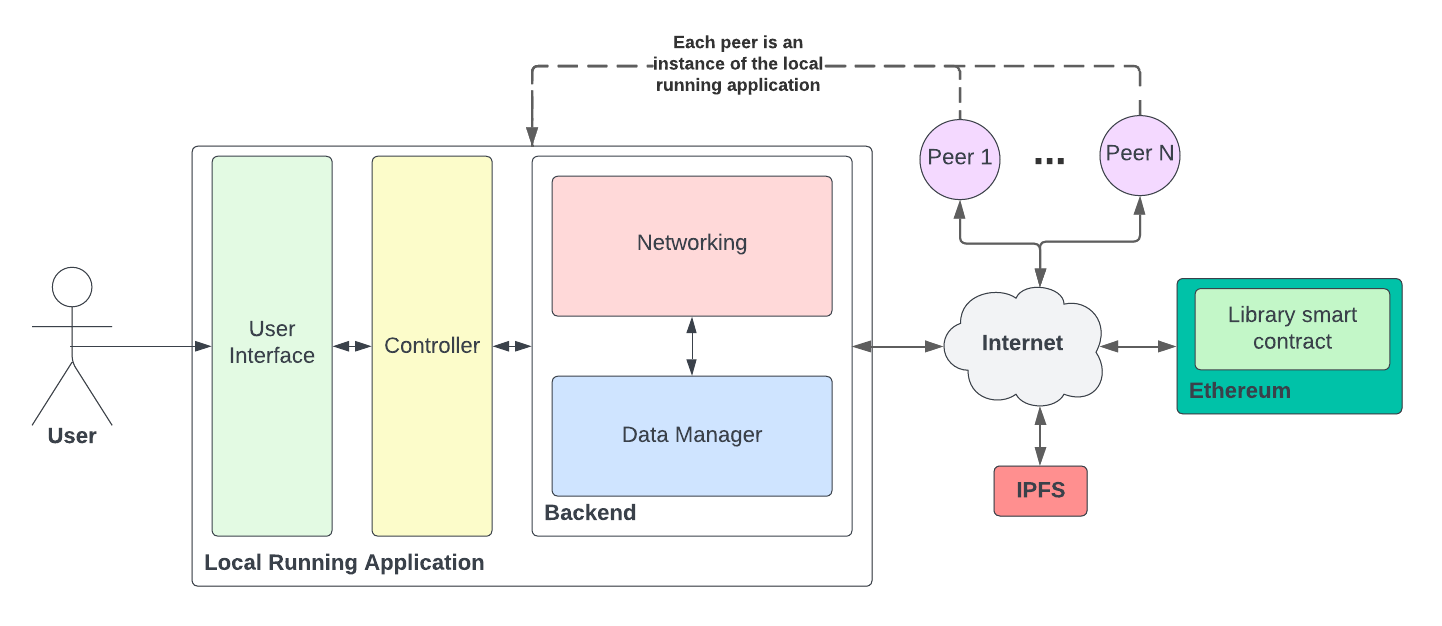
\includegraphics[width=.8\textwidth]{assets/images/diagrams/layers.png}
  \caption{The layers of the application}
  \label{fig:impl-layers}
\end{figure}

% layer entries


\subsection{Persistence}

The Persistence layer shows how the data for the application is divided across several mediums; namely the \textbf{Ethereum Smart Contract}, \textbf{IPFS}, and a \textbf{P2P Network}. Each component stores a different, which is outlined in Section~\ref{subsec:design-data}.
\x
There are several things to note about using Ethereum as platform for selling games:

\begin{itemize}
  \item Ethereum is a less stable currency than most traditional currencies like GBP or USD so games may fluctuate largely in price.
  \item All write functions on the smart contract will incur a gas fee so uploading or updating data will not be free.
  \item Users will have to source Ether from elsewhere before being able to purchase games, which may be intimidating to users not already familiar with the ecosystem.
\end{itemize}

% \subsubsection{Ethereum}\label{subsubsec:impl-eth}

% An Ethereum Smart Contract, written in Solidity \url{https://docs.soliditylang.org/en/v0.8.19/}, will be used to store the set of data about games that is required for the identification of each game. The Smart Contract will also be used to perform the following:
% \x
% The Geth go-ethereum package \url{https://geth.ethereum.org/} will allow us to interact with the ethereum blockchain and Abigen \url{https://docs.avax.network/specs/abigen} will allow us to compile any smart contracts to Go code. This will allow us to interact with our smart contract on ethereum using a set of Go functions. For development, Ganache \url{https://github.com/trufflesuite/ganache} was used to create a local Ethereum instance and Geth was used to connect to an Ethereum test net.


% \subsubsection{IPFS}

% This project will use the IPFS implementation Kubo \url{https://github.com/ipfs/kubo}, due to it being the most widely used implementation of IPFS. We will use the go-ipfs-api library \url{https://github.com/ipfs/go-ipfs-api} to interact with Kubo and upload/download the data specified above.


\subsection*{Backend}\label{subsec:backend}

The Backend can be broken down into two major components:

\begin{itemize}
  \item \textbf{Networking} The creation and maintenance of network connections with other peers over the internet with the purpose of sharing data.
  \item \textbf{Data Manager} the management of local data and the processing of data received and to be uploaded by the Networking component.
\end{itemize}

\input{sections/5-design/components/backend/networking.tex}
\input{sections/5-design/components/backend/manager.tex}
\input{sections/5-design/components/backend/optimisations.tex}

\subsection{User Interface}\label{subsec:ui}

\input{sections/6-implementation/layers/ui/frontend.tex}
\input{sections/6-implementation/layers/ui/controller.tex}

\chapter{Testing}

\newpage
\section{Design Considerations}

% chktex-file 24
% chktex-file 8

\subsection{Data}
\label{subsec:design-data}

Table~\ref{tab:data} discusses the different types of data we are going to need to store and where they should be stored based upon their properties.


\begin{longtable}{ p{.12\textwidth} p{.1\textwidth} p{.1\textwidth} p{.63\textwidth} }
  \toprule
  \textbf{Data} & \textbf{Size} & \textbf{Location} & \textbf{Explanation}\\
  \midrule\midrule
  Game Metadata\newline\reqref{F-M1}
  & 100 -- \newline200B
  & Ethereum
  & This data is the minimal set of information required for the unique identification of each game. See Section~\ref{subsubsec:eth-data}.

  \vspace{1mm}
  This data is appropriate to store on Ethereum as it is public, small in size, and essential to the correct functioning of the application as all users will need to be able to discover all games. 
  \x
  Game Hash Tree\newline\reqref{F-M12}
  & \~15KB
  & IPFS
  & This will be the compressed Hash Tree that will allow the users to identify and verify the shards of data they need to download for their game. The user will download this immediately after purchasing the game.

  \vspace{1mm}
  This data would be costly to store on Ethereum for a large number of games and will only need to be accessed by a subset of users. As it is also public data, IPFS is appropriate to store it on, and we can reference the CID within the data stored on Ethereum.
  \x
  Game\newline Assets\newline\reqref{F-C2}
  & Unkown~\footnote{Some games may include many promotional materials, whilst some could include none. Therefore, it is hard to estimate the expected size.} 
  & IPFS
  & This will represent any promotional material provided for the game that can be viewed on the game's store page. This will typically include cover art and a markdown file for the description. The user will download this when they first view it in the store.

  \vspace{1mm}
  Similar to the Hash Tree, this will typically be too large to store on Ethereum so, given that it is public and non-essential data, IPFS will be used to store and distribute it. 
  \x
  Game Data
  & \textit{avg. 44GB~\footnote{Calculated based off of the top 30 games from SteamDB~\cite{noauthor_steam_nodate}.}}
  & Peers
  & This will the data required to play the game and will be fetched based upon the contents of the game's Hash Tree.

  \vspace{1mm}
  This data is way too large to store on Ethereum but also isn't public, which means using IPFS would not be appropriate~\footnote{IPFS and similar platforms provide no access control for the data stored there and any encryption based technique would be unviable.}. Therefore, this project will use a custom P2P network for sharing data, which is described in Section~\ref{subsec:design-p2p} 
  \\\bottomrule\bottomrule
  \caption{The different types of data required for each game.}
  \label{tab:data}
\end{longtable}

\noindent 
Swarm~\cite{hartman_swarm_1999} was considered as a decentralised storage and distribution platform over IPFS but was decided against as it would couple this project more tightly with Ethereum. On top of that, IPFS has much greater adoption and is much more mature in terms of working on a large scale.
\subsection*{Architecture}

Figure~\ref{fig:architecture-diagram} shows the architecture of this application:

\begin{figure}[ht]
  \centering
  \includegraphics*[width=\textwidth]{assets/images/diagrams/architecture-diagram.png}
  \caption{Architecture of the application}
  \label{fig:architecture-diagram}
\end{figure}

\subsection*{Sequence Diagram}

Figure~\ref{fig:sequence-diagram}, shows the main interactions between actors in the application.

\begin{figure}[ht]
  \centering
  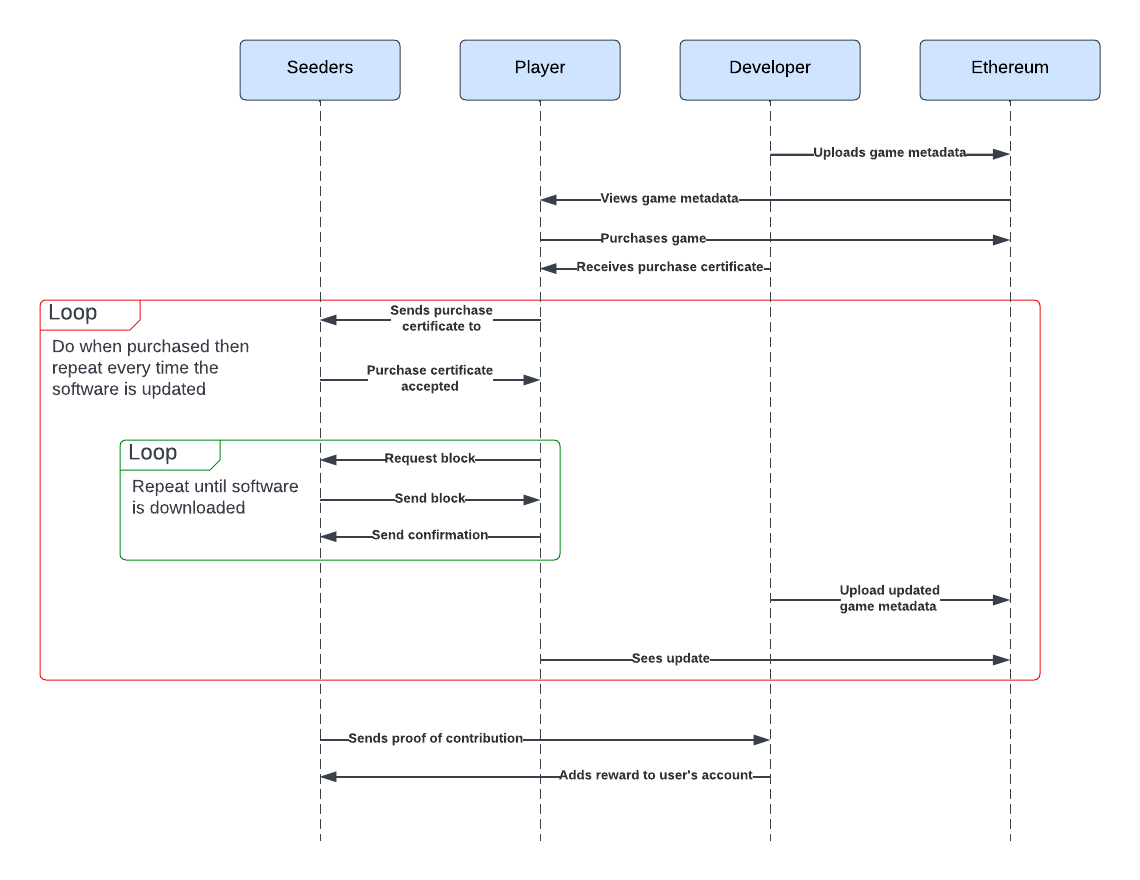
\includegraphics[width=.95\textwidth]{assets/images/diagrams/seqeunce-diagram.png}
  \caption{A sequence diagram showing some of the main interactions within this application}
  \label{fig:sequence-diagram}
\end{figure}



\subsection*{Blockchain}\label{subsec:design-con-eth}

\subsubsection*{Type of Blockchain}

To satisfy \reqref{NF-M1} and \reqref{NF-M2}, we will need to use a public blockchain. This will benefit my project by:
\vspace{2mm}
\begin{itemize}
  \item being accessible to more users, which will boost both availability and scalability \reqref{NF-S1},
  \item reducing the risk of censorship \reqref{NF-M1}, and
  \item providing greater data integrity \reqref{NF-M4}
\end{itemize}

\newparagraph Ethereum is a public blockchain that allows developers to publish their own distributed applications to it. It comes with an extensive development toolchain so is an obvious choice for this project \reqref{F-M4}.

\subsubsection*{Uploading Games}
\label{subsubsec:eth-data}



To satisfy \reqref{F-M1} and \reqref{F-M2}, the data stored on the blockchain will be used for the identification of games. Table~\ref{tab:eth-data} shows the fields that will stored as part of the smart contract for each game and to manage the whole collection of games. Fields in \textit{italics} are generated for the user and non-italic fields are entered manually.

\begin{longtable}{ p{.2\textwidth} p{.75\textwidth} }
  \toprule
  \textbf{Name} & \textbf{Description}
  \\\midrule\midrule
  \multicolumn{2}{c}{\textit{Metadata for each game}} 
  \\\midrule\midrule
  title & The name of the game.\\
  version & The version number of the game.\\
  \textit{release date} & The timestamp for when the game was uploaded.\\
  developer & The name of the developer uploading the game \reqref{NF-M3}.\\
  \textit{uploader} & The Ethereum address of the developer \reqref{NF-M3}.\\
  \textit{root hash} & The root hash of the game that uniquely identifies the game and is based upon its contents.\\
  previous version & The root hash of the most previous version of the game if it exists.\\
  price & The price of the game in Wei.\\
  \textit{hash tree CID} & Required for downloading the hash tree from IPFS.\\
  \textit{assets CID} & Required for downloading the assets folder from IPFS.
  \\\midrule\midrule
  \multicolumn{2}{c}{\textit{Managing the Collection of Games}} 
  \\\midrule\midrule
  \textit{library} & A mapping for all games uploaded to the network, where a game's root hash is the key used to find its metadata.\\
  \textit{game hashes} & Solidity doesn't allow us to enumerate maps so we will also store a list of hashes for all games uploaded.\\
  \textit{purchased} & A mapping which allows us to easily check if a user has purchased a game \reqref{F-M6}.
  \\\bottomrule\bottomrule
  \caption{the data to be stored on Ethereum using a smart contract}
  \label{tab:eth-data}
\end{longtable}


\subsubsection*{Purchasing Content}

Users will purchase games from developers over Ethereum by transferring Ether \reqref{F-M5}. The user's address will then be added to a public record, on the smart contract, of all users who have purchased the game \reqref{F-M6}. Upon purchasing a game, a user will broadcast their new library to all of their peers.

% chktex-file 1
% chktex-file 13

\subsection{Distributed File Sharing}
\label{subsec:design-p2p}

\subsubsection*{Hash Tree}
\label{subsubsec:hash-tree}

The hash tree of a given directory is used to represent its structure as well as the contents of its files. Each file is represented by an ordered list of SHA-256 hashes that match a fixed-size block of data. This allows users to easily identify and verify game data \reqref{F-M10}.

\begin{figure}[ht]
  \centering
  \includegraphics[width=.85\textwidth]{assets/images/diagrams/block-body.png}
  \caption{The structure of a hash tree}
  \label{fig:hash-storage}
\end{figure}

\subsubsection*{Uploading Content}
\label{subsubsec:upload-content}

For a developer to upload their game \reqref{F-M1}, they must provide the following:

\begin{itemize}
  \item the metadata outlined in Section~\ref{subsubsec:eth-data},
  \item a hash tree created from the root directory of the game, and
  \item an assets folder containing a piece of cover art \textit{(cover.png)} and a description file \textit{(description.md)}.
\end{itemize}

\vspace{2mm}\noindent
The developer should be able to enter the required fields into an upload page of the GUI and have the data generated and uploaded for them \reqref{F-S2}.

\subsubsection*{Downloading Content}

\newcommand{\seeder}{$P_{seeder}$~}
\newcommand{\downloader}{$P_{downloader}$~}

Like mentioned in Section~\ref{subsec:design-data}, it is impractical to store the game's data on the blockchain or IPFS. Instead we will consider ideas from decentralised file-sharing networks, like discussed in Sections~\ref{sec:lit-p2p} \&~\ref{sec:bittorrent}.
\x
Games are content addressable using their root hash field, which will allow users to request data from that game from other users. When a peer seeking data \downloader forms a connection with another peer \seeder they will:

\begin{enumerate}
  \item Perform a handshake to determine each other's Ethereum address and public key.
  \item \seeder will verify that \downloader owns the game by checking the \textit{purchased} mapping on the smart contract \reqref{F-M6} \reqref{F-S1}.
  \item \downloader will send requests for individual blocks to \seeder \reqref{F-M9}.
  \item Upon receiving a block, \downloader will verify the contents using the block's hash \reqref{F-M10} before writing it to disk in the appropriate location.
  \item Repeat Steps 3--4 until the entire game has been downloaded \reqref{F-M11}.
  \item \seeder may request a signed receipt that details the blocks they uploaded \reqref{F-S3} to \downloader.
\end{enumerate}

\vspace{2mm}\noindent
Users will be able to connect to many peers at once \reqref{F-M7} and will send download requests to the subset of their peers who also own the game. Requests will be sent in a round-robin fashion to evenly distribute the requests and prevent overloading a single peer \reqref{NF-S1}. Requests that cannot be completed will be retried when connecting to a new peer or when a peer has a change in library.

\subsubsection*{Updating Content}\label{subsubsec:updating}

To satisfy \reqref{F-M2}, developers will perform the same steps outlined in Section~\ref{subsubsec:upload-content} but must also provide the root hash of the most previous version of the game. Any users who have purchased the previous version will be added to the list of users who have purchased the new version \reqref{F-M3}. Additionally, this will include the restriction that only the original uploader can upload an update for their game \reqref{NF-M5}.
\x
Each version is considered its own game and will require users to download the updated version separately. Whilst this isn't reflective of how updates are typically managed, this will be acceptable for the scope of this project.

\subsubsection*{Downloadable Content}

Downloadable Content (DLC) \reqref{F-C1} represent optional additions for games that users will buy separately. DLCs will act similarly to how updates are treated. Each DLC will need:

\begin{enumerate}
  \item \textbf{Dependency} The root hash of the oldest version of the game this DLC supports.
  \item \textbf{Previous Version} (Optional) The root hash of the previous version of the DLC.
\end{enumerate}

\vspace{2mm}\noindent
Users must own the original game to buy any of its DLC. 

\subsubsection*{Proving Contribution}

As a user downloads blocks of data, they will keep track of which users have sent them which blocks. A peer may then request their contributions in the form of a signed message that can be sent to the developer \reqref{F-S3} in return for some kind of reward. The contents of the reward isn't specified for this project but could include in-game items, digital assets or Ether. This solution assumes that developers have knowledge of which Ethereum address maps to which of their game's users.
\section{Unit Testing}

Unit tests were written alongside the code they were testing to ensure my code was robust and responded appropriately to all inputs. I aimed for a 70\% test coverage to ensure a significant amount of the application was tested. Table~\ref{tab:coverage} shows a breakdown of test coverage by package.

\begin{longtable}{p{.4\textwidth} p{0.15\textwidth} p{.2\textwidth}}
  \toprule
  \textbf{Package} & \textbf{Coverage} & \textbf{Tests Written}
  \\\midrule\midrule
  model/manager/hashtree
  & 75.2\%
  & 69
  \\
  model/manager/games
  & 61.3\%
  & 107
  \\
  model/manager/ignore
  & 90.6\%
  & 13
  \\
  model/net/tcp
  & 70.1\%
  & 23
  \\
  model/net/peer
  & 53.7\%
  & 154
  \\
  model/persistence/ethereum
  & 81.7\%
  & 20
  \\
  model/util
  & 61.2\%
  & 24
  \\\midrule\midrule
  \textbf{Total}
  & 70.5\%
  & 410
  \\\bottomrule\bottomrule
  \caption{Code coverage by package. Missing entries do not have code in them for example model/manager is only a wrapper for its child packages.}
  \label{tab:coverage}
\end{longtable}

\newparagraph
Automated tests were also written for the smart contract functions and tested locally using Ganache CLI~\cite{noauthor_trufflesuiteganache_2023}. 
Tests were not written for generic functions like getters and setters; this includes the Controller functions that were typically wrappers around Backend functions. Equally, automated UI tests were omitted due to time constraints and that UI components were partially tested by the user walkthroughs.
\section{Integration Testing}

\subsection*{Profiles}

A profile is used to mimic a specific type of peer that a user may find through this application. This is to allow me to test my application under different conditions and see how it reacts. Table~\ref{tab:profiles} details the used profiles.

\small
\begin{longtable}{p{.15\textwidth} p{.7\textwidth}}
  \toprule
  \textbf{Name} & \textbf{Purpose}
  \\\midrule\midrule
  \textbf{Listen Only}
  & A peer who will listen and respond to all requests perfectly but will never request anything. This is useful for testing when we want a lightweight client to just download data off of. 
  
  This will also be able to upload a game to the locally running smart contract.
  \\
  \textbf{Sender}
  & This peer will respond to requests but will also periodically send requests. This can be used to show how my application reacts to more realistic peers. 
  \\
  \textbf{Unreliable}
  & This peer will pseudo-randomly not respond to messages or send incorrect data in response. This is used to show how my application recovers from faults sent by other users.
  \\
  \textbf{Selfish}
  & This peer will send requests but will never respond to any. This is used to show how my application handles expired requests.
  \\\bottomrule\bottomrule
  \caption{The different profiles used to simulate real-world peers.}
  \label{tab:profiles}
\end{longtable}
\normalsize

\noindent
The main outcome from these different profiles shows the need for a reputation system where a user can distinguish between peers that reliably respond to requests and peers that don't. This would help mitigate some of the overhead of timed-out requests or receiving incorrect data.

% chktex-file 44

\newpage
\section{Benchmarking}\label{sec:benchmark}

Benchmarking is being used in this project to determine the overall performance and scalability of the application, whilst also being useful in identifying any bottlenecks or how the end user can optimise their inputs. The key benchmark being assessed is related to how the application scales downloading games by varying the following factors:

\begin{enumerate}
  \item how many of the peers we are connected to have the data we need,
  \item how large is the game (in terms of average file size and number of files), and
  \item the shard size used to create the hash tree.
\end{enumerate}

\vspace{2mm}\noindent
To ensure the consistency and correctness of results, all benchmarks will be ran on the same machine, running the same OS, and be completed multiple times. The test data is a collection of pseudo-randomly generated files that meet the criteria specified in each benchmark. Moreover, the project size used for all benchmarks will be 40GB to match the average game size given in Section~\ref{subsec:design-data}.

\subsection*{Number of Peers}

This benchmark allows us to observe how the application scales when dealing with many peers at the same time and how if affects the overall performance of the application.
\x
For each run, we will create a project with 500 files, each of size 80MB and a shard size of $2^{22}$ = 4MiB. We will then run $N$ peers locally to simulate a perfect network connection.

\begin{longtable}{l|llll|}
  \cline{2-5}
  & \multicolumn{4}{c|}{\hdr{Runtime (s)}}                                                    \\ \hline
  \multicolumn{1}{|l|}{\hdr{Peer Count}} 
  & \multicolumn{1}{l|}{\hdr{1}} 
  & \multicolumn{1}{l|}{\hdr{2}} 
  & \multicolumn{1}{l|}{\hdr{3}} & \hdr{avg.}  \\ \hline
  \multicolumn{1}{|l|}{1} & 
  \multicolumn{1}{l|}{56} & 
  \multicolumn{1}{l|}{65} & 
  \multicolumn{1}{l|}{63} &  
  61.3
  \\ \hline
  \multicolumn{1}{|l|}{2} & 
  \multicolumn{1}{l|}{65} & 
  \multicolumn{1}{l|}{64} & 
  \multicolumn{1}{l|}{60} &  
  63
  \\ \hline
  \multicolumn{1}{|l|}{4} & 
  \multicolumn{1}{l|}{66} & 
  \multicolumn{1}{l|}{65} & 
  \multicolumn{1}{l|}{65} &  
  65.7
  \\ \hline
  \multicolumn{1}{|l|}{8} & 
  \multicolumn{1}{l|}{66} & 
  \multicolumn{1}{l|}{62} & 
  \multicolumn{1}{l|}{60} &  
  62.7
  \\ \hline
  \caption{How varying peer count affects download speed}
\end{longtable}

\noindent Taking into account a degree of error, it is clear that increasing the number of peers does not reduce the download time. This indicates that a bottleneck may exist elsewhere in the application such as inserting received data. This is supported by the observation that downloads got much slower towards the end and would often take \~15 seconds for the last 10\%; however, this could also be caused by the file verification that is ran once an entire file is downloaded.
\x
However, this result also shows that many peers can be supported without an impact on performance. However, maintaining TCP connections will be expensive for a very large number of peers so a UDP implementation should be a consideration moving forward. 

\subsection*{Game Size}

This benchmark will be useful in discovering an optimal strategy for determining the directory structure of games uploaded to the network to allow developers to optimise their uploads to give the greatest download speed. 
\x
For each run, we will create a project with $F$ files of size $S$MB, such that $F\times S = 40GB$, and a shard size of 4MiB. We will then run 1 peer locally to simulate a perfect network connection.

\begin{longtable}{rr|llll|}
  \hline
  \multicolumn{2}{|c|}{\hdr{File}}
  & \multicolumn{4}{c|}{\hdr{Runtime (s)}}
  \\\hline
  \multicolumn{1}{|l|}{\hdr{Count}} 
  & \hdr{Size (MB)}
  & \multicolumn{1}{l|}{\hdr{1}} 
  & \multicolumn{1}{l|}{\hdr{2}} 
  & \multicolumn{1}{l|}{\hdr{3}} 
  & \hdr{avg.}
  \\ \hline
  \multicolumn{1}{|r|}{200} 
  & 200
  & \multicolumn{1}{l|}{57} 
  & \multicolumn{1}{l|}{55} 
  & \multicolumn{1}{l|}{58} 
  &  57
  \\\hline
  \multicolumn{1}{|r|}{100} 
  & 400
  & \multicolumn{1}{l|}{56} 
  & \multicolumn{1}{l|}{52} 
  & \multicolumn{1}{l|}{58} 
  & 55
  \\\hline
  \multicolumn{1}{|r|}{50} 
  & 800
  & \multicolumn{1}{l|}{} 
  & \multicolumn{1}{l|}{} 
  & \multicolumn{1}{l|}{} 
  &  
  \\\hline
  \multicolumn{1}{|r|}{25} 
  & 1,600
  & \multicolumn{1}{l|}{} 
  & \multicolumn{1}{l|}{} 
  & \multicolumn{1}{l|}{} 
  &  
  \\\hline
  \multicolumn{1}{|r|}{5} 
  & 8,000
  & \multicolumn{1}{l|}{} 
  & \multicolumn{1}{l|}{} 
  & \multicolumn{1}{l|}{} 
  &  
  \\\hline
  \multicolumn{1}{|r|}{1} 
  & 40,000
  & \multicolumn{1}{l|}{} 
  & \multicolumn{1}{l|}{} 
  & \multicolumn{1}{l|}{} 
  &  
  \\\hline
  \caption{How varying file count and size affects download speed}
\end{longtable}

\subsection*{Shard Size}

This benchmark will be useful in determining an optimal shard size to use that maximises download speed.
\x
For each run we will create a new project with 500 files, each of size 80MB, and a shard size of $B$MiB. We will then run 1 peer locally to simulate a perfect network connection.

\begin{longtable}{r|llll|}
  \cline{2-5}
  & \multicolumn{4}{l|}{\hdr{Runtime (s)}}
  \\ \hline
  \multicolumn{1}{|l|}{\hdr{Shard Size (bytes)}} 
  & \multicolumn{1}{l|}{\hdr{1}} 
  & \multicolumn{1}{l|}{\hdr{2}} 
  & \multicolumn{1}{l|}{\hdr{3}} 
  & \hdr{avg.}
  \\\hline
  \multicolumn{1}{|r|}{1,048,576} 
  & \multicolumn{1}{l|}{} 
  & \multicolumn{1}{l|}{} 
  & \multicolumn{1}{l|}{} 
  & 
  \\\hline
  \multicolumn{1}{|r|}{2,097,152} 
  & \multicolumn{1}{l|}{} 
  & \multicolumn{1}{l|}{} 
  & \multicolumn{1}{l|}{} 
  & 
  \\\hline
  \multicolumn{1}{|r|}{4,194,304} 
  & \multicolumn{1}{l|}{} 
  & \multicolumn{1}{l|}{} 
  & \multicolumn{1}{l|}{} 
  & 
  \\\hline
  \multicolumn{1}{|r|}{8,388,608} 
  & \multicolumn{1}{l|}{} 
  & \multicolumn{1}{l|}{} 
  & \multicolumn{1}{l|}{} 
  & 
  \\\hline
  \multicolumn{1}{|r|}{16,777,216} 
  & \multicolumn{1}{l|}{} 
  & \multicolumn{1}{l|}{} 
  & \multicolumn{1}{l|}{} 
  & 
  \\\hline
  \caption{How varying the shard size of the hash tree affects download speed}
\end{longtable}
% chktex-file 44

\section{Acceptance Testing}\label{sec:acc-tests}

A user walkthrough is a series of steps to take that, if completed, prove the completeness of a set of requirements. Table~\ref{tab:walkthroughs} describes all user walkthroughs and Appendix~\ref{app:user-walkthrough} shows the evidence for their completeness.
All user walkthroughs use a contract deployed to the Sepolia test-net~\cite{etherscanio_library_nodate}, satisfying \reqref{F-M4}, \reqref{NF-M2} and \reqref{NF-M1}. I have also uploaded the smart contract source code to demonstrate that specific functions are called following specific events. 

\newcommand{\p}[1]{$P_{#1}$}
\newcommand{\g}[1]{$G_{#1}$}

\small
\begin{longtable}{ p{.02\textwidth} p{.2\textwidth} p{.56\textwidth} p{0.1\textwidth} }
  \toprule
  \textbf{Id} & \textbf{Requirements} & \textbf{Description} & \textbf{Success}\\\midrule\midrule
  1
  & \reqref{F-M1} \reqref{F-M5} \reqref{F-M12} \reqref{F-S2} \reqref{F-C2} \reqref{NF-M3}
  & \vspace{-5mm}\begin{enumerate}[wide, labelwidth=!, labelindent=0pt]
    \item \p{1} uploads a game \g{1}.
    \item \p{2} finds \g{1} on the store.
    \item \p{2} purchases \g{1}.
    \item \p{2} shows \g{1} added to their library.
  \end{enumerate}
  & \yes
  \\\midrule
  2 
  & \reqref{F-M6} \reqref{F-M8} \reqref{F-M9} \reqref{F-M10} \reqref{F-M11} \reqref{F-S1} \reqref{F-S2} \reqref{F-S3} \reqref{NF-M2} 
  & \vspace{-5mm}\begin{enumerate}[wide, labelwidth=!, labelindent=0pt]
    \item \p{2} connects to \p{1}.
    \item \p{1} and \p{2} exchange Ethereum addresses.
    \item \p{2} starts a download for \g{1}.
    \item \p{2} sends requests for blocks to \p{1}.
    \item \p{1} queries the smart contract to verify that \p{2} owns \g{1}.
    \item \p{1} will respond to \p{2} with the requested data.
    \item \p{2} will verify each block of data received using its hash.
    \item \p{2} will have full downloaded \g{1}.
    \item \p{1} will request and receive a contributions receipt for \g{1} from \p{2}.
  \end{enumerate}
  & \yes
  \\\midrule
  3
  & \reqref{F-M2} \reqref{F-M3} \reqref{F-M6} \reqref{NF-M5}
  & \vspace{-5mm}\begin{enumerate}[wide, labelwidth=!, labelindent=0pt]
    \item \p{1} is the original uploader of \g{1} and \p{2} has already purchased \g{1}.
    \item \p{1} uploads an update to \g{1}, \g{2}.
    \item \p{2} will hit the ‘check for updates’ button and see \g{2} in their library.
  \end{enumerate}
  & \yes
  \\\midrule
  4
  & \reqref{F-S4} \reqref{F-M7} \reqref{NF-M2} 
  & \vspace{-5mm}\begin{enumerate}[wide, labelwidth=!, labelindent=0pt]
    \item \p{1} is connected to \p{2}.
    \item \p{3} forms a connection with \p{1}.
    \item \p{3} requests a list of \p{1}'s peers and \p{1} responds with the details for \p{2}.
    \item \p{4} forms connections with \p{2}.
  \end{enumerate}
  & \yes
  \\\bottomrule\bottomrule
  \caption{The set of user walkthroughs used to prove the completeness of this project's requirements.}
  \label{tab:walkthroughs}
\end{longtable}
\normalsize

\chapter{Project Management}

\section{Gantt Chart}

\begin{figure}[ht]
  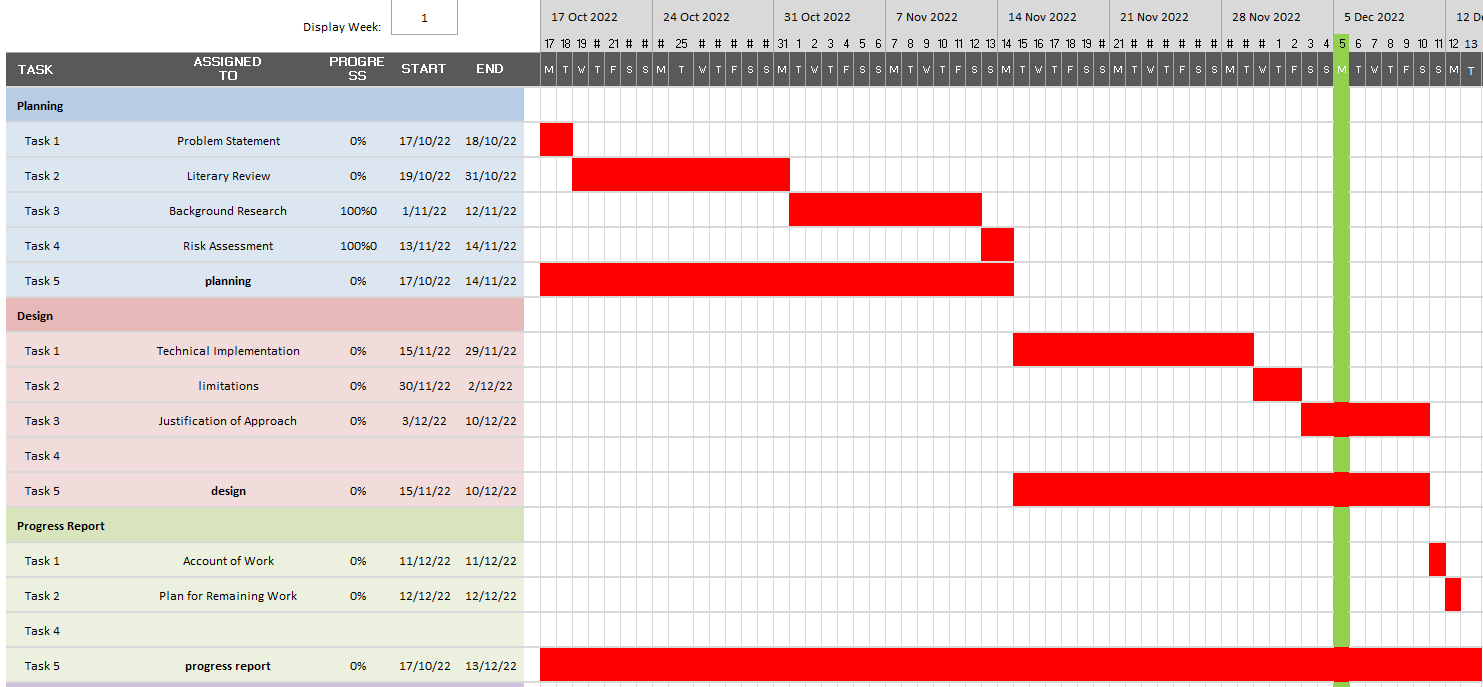
\includegraphics[width=\textwidth]{diagrams/gantt-chart-1.png}
  \caption{\textit{A Gantt chart for my work up until the progress report.}}
\end{figure}

% \begin{figure}[ht]
%   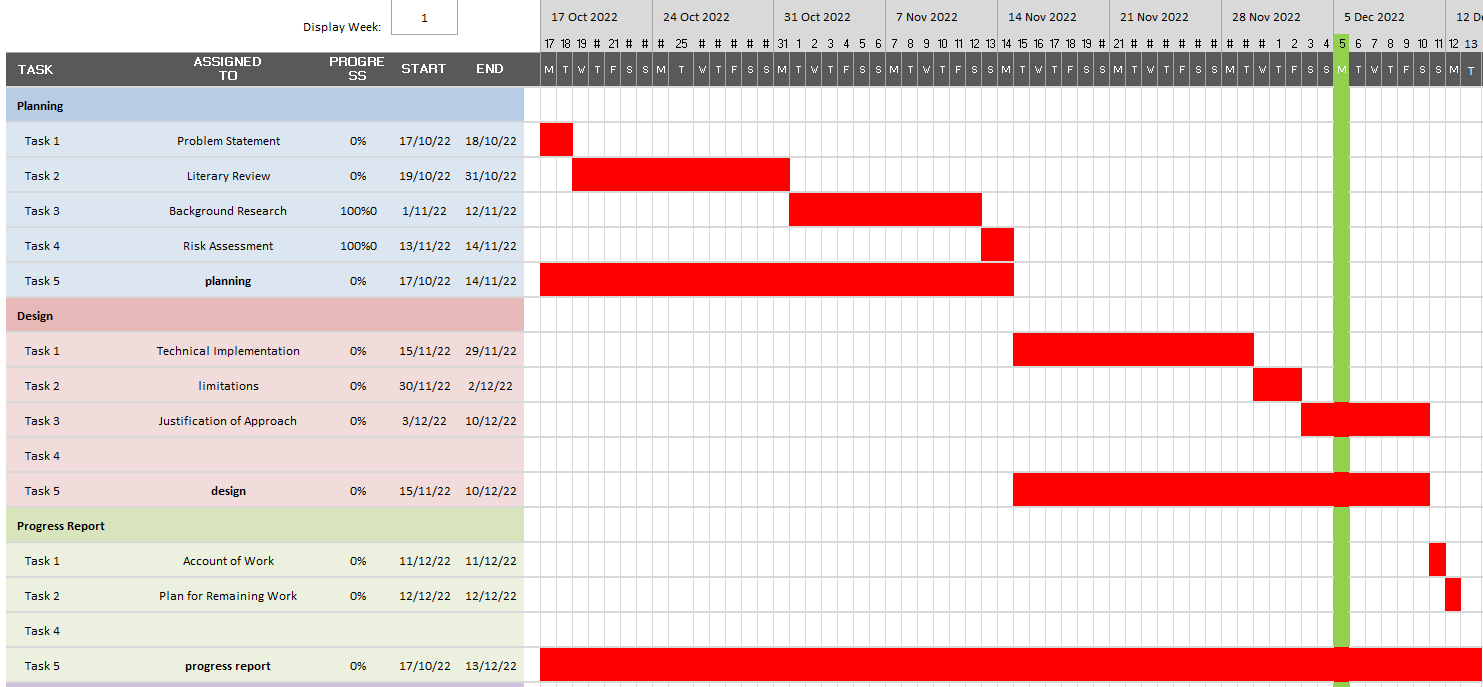
\includegraphics[width=\textwidth]{diagrams/gantt-chart-1.png}
%   \caption{\textit{A Gantt chart for my work by the handin of the progress report.}}
% \end{figure}

\section{Risk Assessment}

\begin{longtable}[ht]{ p{.2\textwidth} p{0.06\textwidth}  p{0.06\textwidth} p{0.06\textwidth} p{0.5\textwidth}}
  \toprule
  \textbf{Risk}
   & \textbf{Loss}
   & \textbf{Prob}
   & \textbf{Risk}
   & \textbf{Mitigation}
  %
  \\\midrule\midrule
  Laptop damaged or lost
   & 3
   & 1
   & \cellcolor{orange!50} 5
   & All work is stored using version control and periodic backups will be
  made and stored locally and in cloud storage. I have other devices that
  could be used to continue development.
  %
  \x
  Difficulty with blockchain development
   & 2
   & 3
   & \cellcolor{orange!50} 6
   & I will seek advice from my supervisor about how to tackle certain problems
  and if necessary, what aspects of my project I should change.
  %
  \x
  The application is not finished
   & 1
   & 3
   & \cellcolor{green!30} 3
   & Using agile development will ensure that I will at least have a minimal
  working application. If I feel that I am running out of time, I will focus
  on expanding test cases and improving the write-up.
  %
  \x
  No suitable large scale test environment
   & 2
   & 5
   & \cellcolor{red!40} 10
   & I do not have the infrastructure to test this project on a large network,
  however small scale tests will be possible.
  %
  \x
  Personal illness
  & 3
  & 2
  & \cellcolor{orange!50} 6
  & Depending on the amount of lost time, I may have to not complete some of the SHOULD or COULD requirements.
  \\\bottomrule\bottomrule
  \\\caption{\textit{The risk assessment of this project.}}
  \label{tab:risk assessment}
\end{longtable}
\chapter{Evaluation}


\section{Stakeholders \& Requirements}


\subsection{Stakeholders}

\newcommand{\primary}{\hlc{cyan}{ PRIMARY }\\}
\newcommand{\secondary}{\hlc{yellow}{ SECONDARY }\\}
\newcommand{\tertiary}{\hlc{green}{ TERTIARY }\\}

\paragraph{Game Developers}\primary
This group will use the application to release their games and its updates to their users, who they will reward for helping to distribute it.

\paragraph{Players}\primary
This group will use this application to downloaded and update their games off of. They may also contribute to the distribution of the games to other players for an incentive provided by the developers.

\paragraph{Game Distribution Platforms}\secondary
This group consists of platforms like Steam or Epic Games, which serve as the main competitor to this application. It is likely that as more developers choose this application, this group will see a loss in revenue. 

\paragraph{}\tertiary

\subsection{Requirements}

Tables~\ref{tab:functional-requirements} and~\ref{tab:non-functional-requirements} show the functional and non-functional requirements of this project organized using MoSCoW prioritisation. 

\subsubsection*{Functional Requirements}

\begin{longtable}{ p{.1\textwidth} p{.8\textwidth} }
  \toprule
  \textbf{ID} & \textbf{Description}
  \\\midrule\midrule
  \multicolumn{2}{c}{\cellcolor{red!70}\textit{Must}}\\\midrule
  F\_M1 & Store software metadata on a blockchain\\
  F\_M2 & A node must request individual shards from its peers\\
  F\_M3 & A node must be able to discover peers relevant to the software it wants\\
  F\_M4 & Software must be updatable through the blockchain\\
  F\_M5 & A node must be able to upload software\\
  F\_M6 & A node must be able to download software in its entirety from nodes in the same network.\\
  F\_M7 & A node must be able to verify the integrity of each block it downloads\\
  F\_M8 & The application should run on the Ethereum network\\
  F\_M9 & Users must be able to purchase games from developers over the network\\
  F\_M10 & Users must be able to prove they have purchased a game\\
  \midrule\multicolumn{2}{c}{\cellcolor{orange!70}\textit{Should}}\\\midrule
  F\_S1 & Seeders should have a way to prove how much data they have seeded\\
  F\_S2 & Seeders will only upload content to users who have a valid proof of purchase\\
  \midrule\multicolumn{2}{c}{\cellcolor{green}\textit{Could}}\\\midrule
  F\_C1 & Allow users to request specific software versions\\
  \midrule
  \bottomrule
  \label{tab:functional-requirements}
\end{longtable}

\subsubsection*{Non-Functional Requirements}

\begin{longtable}{ p{.1\textwidth} p{.8\textwidth} }
  \toprule
  \textbf{ID} & \textbf{Description}
  \\\midrule\midrule
  \multicolumn{2}{c}{\cellcolor{red!70}\textit{Must}}\\\midrule
  NF\_M1 & The application is decentralized and cannot be controlled by any one party\\
  NF\_M2 & Any user must be able to join and contribute to the network\\
  NF\_M3 & Game uploaders should be publicly identifiable\\
  NF\_M4 & Metadata required to download the game should be immutable\\
  \midrule\multicolumn{2}{c}{\cellcolor{orange!70}\textit{Should}}\\\midrule
  NF\_S1 & This application must be scalable, such that many users can upload and download the same game at the same time.\\
  NF\_S2 & Only the original uploader can upload an update to their game\\
  \midrule\multicolumn{2}{c}{\cellcolor{green}\textit{Could}}\\\midrule
  \\
  \midrule
  \bottomrule
  \label{tab:non-functional-requirements}
\end{longtable}
\section{Development}

\subsection{Overview}

\paragraph*{Complexity}
My overall impression of this project was that it was too complex and took a lot more time and effort than was initially expected when planning. Whilst use of agile development helped me organise my time and prioritise features, it still felt like it wasn't enough and that I should have reduced the scope and focused on a more minimal version of the application.



\paragraph*{Test-Driven Development TDD}
TDD was a critical part to the success of this project and helped me catch bugs when writing and extending the application. By having an automated test-suite, I could rapidly test large portions of my codebase and find where potential issues appeared. 
\x
However, one issue with writing tests in Go was that the test libraries used often didn't feel robust enough when compared to libraries from other languages (namely JUnit). To give some examples:

\begin{itemize}
  \item Dependency injection and mocking are much harder in Go and rely on an interface based approach. This would add a large amount of complexity and boilerplate to my codebase for the sake of writing tests. Instead it was generally easier to write tests that relied on several other components unrelated to the tested code.
  \item There is no easy way to configure functions to run before/after all/each test. You can run functions before and after all tests in a package but not individual test files, and before/after each function have to specified in every test they're in. 
  \item Tests are not easily groupable and tags can only be specified per file but not on a test by test basis. The standard package only supports categorising individual tests as \textit{short} or not.
\end{itemize}
\section{Future Work}

\subsection{Optimisations}

There are several changes that we could make to improve the performance of the project as a whole and make the downloading of data more efficient. These include:

\begin{enumerate}
  \item \textbf{New Commands} We could extend the commands described in Section~\ref{subsubsec:commands} by including support for batch block requests. This would allow users to request many blocks at once and avoid the overhead of having to perform one request per block.  
  \item \textbf{Better Block Selection} Currently blocks are not ranked in any way, and by considering the ideas set out in Section~\ref{subsec:bittorrent-download}, we could improve the download speed and overall availability and efficiency of data throughout the network.
  \item \textbf{Represent Data Differently} The main issue with modelling our data as a Hash Tree is that each file needs to have at least one block. This means that for projects with a large amount of small files, we are substantially increasing the download time as blocks are requested one at a time.

  One possible solution would be to represent the directory as a contiguous block of data that contains breakpoints between files and directories that can be indexed. This would mean we could reduce the overall number of blocks and reduce the amount of redundant data sent between nodes.
\end{enumerate}

\subsection{New Features}

\subsubsection{Downloadable Content DLC}
DLC was initially considered as a requirement for this project (\req{F-S3} \& \req{NF-S3}) but was not completed due to time constraints. DLC would be a necessary addition to this application to ensure the viability of it as a competitor to existing platforms. See the potential implementation details specified in Section

\subsubsection{Discovery}

\paragraph*{Content Discovery}
The store aspect of the application is limited in that users have to know the root hash of the game to find the game's store page and purchase it. This could be achieved using several techniques:

\begin{itemize}
  \item \textbf{Indexing} Periodically generate an index of all games uploaded that allows users to easily search the store without having to make a large amount of requests to the blockchain. Games could also be ranked based upon factors like popularity of availability. 
  \item \textbf{More Metadata} Add further metadata to games that allows them to be grouped and thus more easily searchable. For example, developers could add a set of tags to games to identify what type of game it is or what features it has.
\end{itemize}

\paragraph*{Peer Discovery}\label{pg:discovery}
Currently, there is not good way to discover peers who have the content that a user is interested in. This could be implemented using the following:

\begin{itemize}
  \item \textbf{Tracker} BitTorrent uses tracker's to store a list of peers who are interested in a particular piece of data. A similar technique could be implemented to allow users to easily find new peers but would require this data to be hosted somewhere.
  \item \textbf{Neighbour Discovery} Query known peers if they know any users who are interested in a particular piece of content. However given that the network is fragmented, there is no guarantee that a peer could be found this way.
\end{itemize}

\subsubsection{Streamline Updates}

At the moment, each update to a game is considered as a new game entirely and this has the limitation that a user will have to download the entirety of the game again and not just the updated sections. This also doesn't overwrite any existing data so the user will have to manually uninstall the older version.
\x
A future improvement would be to streamline this process so that for a given update, only the changed data is downloaded and it is overwritten in-place on the older version of the game. This would drastically reduce the bandwidth requirement for each update and require less manual work from the user.


\chapter{Conclusion}

\section*{Conclusion}

This project set out to demonstrate how video game distribution could be migrated to a distributed platform with the aim of reducing the risk of censorship, improving ownership and increasing profits for developers.
\x
By researching related topics and reviewing the literature around key areas of this project, I was able to combine many modern ideas and techniques to develop a functional proof-of-concept application. The heavy use of automated testing allowed me to continuously write robust and correct code.
\x
As most of the requirements set out in Section~\ref{subsec:requirements}, I can say that this project was successful in providing a proof-of-concept application t
\section{Future Work}

\subsection{Optimisations}

There are several changes that we could make to improve the performance of the project as a whole and make the downloading of data more efficient. These include:

\begin{enumerate}
  \item \textbf{New Commands} We could extend the commands described in Section~\ref{subsubsec:commands} by including support for batch block requests. This would allow users to request many blocks at once and avoid the overhead of having to perform one request per block.  
  \item \textbf{Better Block Selection} Currently blocks are not ranked in any way, and by considering the ideas set out in Section~\ref{subsec:bittorrent-download}, we could improve the download speed and overall availability and efficiency of data throughout the network.
  \item \textbf{Represent Data Differently} The main issue with modelling our data as a Hash Tree is that each file needs to have at least one block. This means that for projects with a large amount of small files, we are substantially increasing the download time as blocks are requested one at a time.

  One possible solution would be to represent the directory as a contiguous block of data that contains breakpoints between files and directories that can be indexed. This would mean we could reduce the overall number of blocks and reduce the amount of redundant data sent between nodes.
\end{enumerate}

\subsection{New Features}

\subsubsection{Downloadable Content DLC}
DLC was initially considered as a requirement for this project (\req{F-S3} \& \req{NF-S3}) but was not completed due to time constraints. DLC would be a necessary addition to this application to ensure the viability of it as a competitor to existing platforms. See the potential implementation details specified in Section

\subsubsection{Discovery}

\paragraph*{Content Discovery}
The store aspect of the application is limited in that users have to know the root hash of the game to find the game's store page and purchase it. This could be achieved using several techniques:

\begin{itemize}
  \item \textbf{Indexing} Periodically generate an index of all games uploaded that allows users to easily search the store without having to make a large amount of requests to the blockchain. Games could also be ranked based upon factors like popularity of availability. 
  \item \textbf{More Metadata} Add further metadata to games that allows them to be grouped and thus more easily searchable. For example, developers could add a set of tags to games to identify what type of game it is or what features it has.
\end{itemize}

\paragraph*{Peer Discovery}\label{pg:discovery}
Currently, there is not good way to discover peers who have the content that a user is interested in. This could be implemented using the following:

\begin{itemize}
  \item \textbf{Tracker} BitTorrent uses tracker's to store a list of peers who are interested in a particular piece of data. A similar technique could be implemented to allow users to easily find new peers but would require this data to be hosted somewhere.
  \item \textbf{Neighbour Discovery} Query known peers if they know any users who are interested in a particular piece of content. However given that the network is fragmented, there is no guarantee that a peer could be found this way.
\end{itemize}

\subsubsection{Streamline Updates}

At the moment, each update to a game is considered as a new game entirely and this has the limitation that a user will have to download the entirety of the game again and not just the updated sections. This also doesn't overwrite any existing data so the user will have to manually uninstall the older version.
\x
A future improvement would be to streamline this process so that for a given update, only the changed data is downloaded and it is overwritten in-place on the older version of the game. This would drastically reduce the bandwidth requirement for each update and require less manual work from the user.



%% END OF SECTIONS 

\ifbodyonly 
\else

\newpage
\chapter{References}

\printbibliography[heading=subbibintoc, title={Peer-to-Peer File Sharing}, keyword=p2p]
\printbibliography[heading=subbibintoc, title={Blockchain}, keyword=report-blockchain]
\printbibliography[heading=subbibintoc, title={Tools Used}, keyword=tool]
\printbibliography[heading=subbibintoc, title={Project Management}, keyword=project-management]

\printbibliography[heading=subbibintoc, title={Other}, notkeyword=report-blockchain, notkeyword=p2p, notkeyword=tool,notkeyword=project-management]

\appendix


\chapter{User Walkthroughs}\label{app:user-walkthrough}

This section will go through each of the acceptance tests outlined in Section~\ref{sec:acc-tests} and provide the evidence that they pass. This evidence will be given in the form of:

\begin{itemize}
  \item Smart contract transaction logs from the Sepolia test-net. These are public at \small\url{https://sepolia.etherscan.io/address/0x2899dab55a4a20d698062bbf4d4ce9f1073ce052}\normalsize. The smart contract code was uploaded so all functions called and data uploaded are visible.
  \item Snippets of logs written that correspond to certain actions. For example, receiving a message over the network.
  \item Screenshots to show changes being reflected in the user interface.
\end{itemize}

\newparagraph
For this the game will be a simple folder of text files that we can easily compare to show correctness.

\small
\begin{itemize}
  \item \g{1} = [title="User WT", version="1.0", developer="tcs1g20",\newline uploader=0xfBC8D99Bb9ab8F781fF04F9b45Fe5c97AACE1916, previousVersion=None, price=0, rootHash=`']
  \item \g{2} = [title="User WT", version="2.0", developer="tcs1g20", previousVersion=\g{1}, price=0,\newline uploader=0xfBC8D99Bb9ab8F781fF04F9b45Fe5c97AACE1916, rootHash=`']
\end{itemize}
\normalsize


\chapter{Introduction}\label{sec:problem}

Millions of worldwide users enjoy video games, which are large pieces of software that require complex platforms to distribute them, which results in them being generally provided by multinational corporations. However this approach often results in these platforms:

\begin{itemize}
  \item taking a large cut of revenue from developers\footnote{Steam take a 30\% cut~\cite{marks_report_2019,brown_valve_2021}},
  \item being prone to censorship from entities like governments\footnote{See the Chinese version of Steam~\cite{noauthor_steam_nodate-1}},
  \item relying on a single platform to stay active, distribute games and maintain a user's ownership\footnote{The Nintendo eShop closing down prevents users from accessing games~\cite{noauthor_nintendo_2022}}.
\end{itemize}

\section{Objectives}

Modern web ideas revolve around taking power away from large corporations and having platforms that are built, run and maintained by those who use them.
This project aims to produce a proof-of-concept, distributed video game marketplace that will allow developers to continuously release and update their games on a public network such that they can be purchased and downloaded by other users.

\section{Scope}

This project will strictly focus on creating a distributed platform in which users can upload, purchase and share games and will consist of the following components:

\begin{enumerate}
  \item An Ethereum smart contract that will allow us to maintain a library of games that can be queried and added to by any user. This will then be deployed to an Ethereum test-net.
  \item A local application to be run by users to interact with the smart contract and allow them to join a peer-to-peer network where they can download and upload games.
\end{enumerate}

\newparagraph
This project will not present methods for preventing or stopping the distribution of illegal content or include tangentially related features such as achievements, or message boards.

\chapter{Background Research}

This chapter describes two distributed-web technologies that allows user to connect over large, decentralised networks and overcome issues of distributing data and building trust.

\input{sections/2-background-research/bittorrent.tex}
\input{sections/2-background-research/ethereum.tex}

\chapter{Project Management}

\input{sections/3-project-management/risks/risks.tex}
\input{sections/3-project-management/sprints.tex}
\input{sections/3-project-management/gantt.tex}
% \input{sections/3-project-management/work-to-date.tex}
% \input{sections/3-project-management/plan.tex}

\chapter{Literature Review}\label{ch:lit-review}

This section will be used to examine the literature surrounding the distributed storage of data. Initially I will look at various distributed file-sharing protocols and then how blockchain has been used to enhance them.

\input{sections/4-lit-review/file-sharing.tex}
\input{sections/4-lit-review/cloud-storage.tex}

\section{Overview}
\chapter{Design}

\input{sections/5-design/analysis/analysis.tex}
\input{sections/5-design/considerations/considerations.tex}
\input{sections/5-design/components/components.tex}
\input{sections/5-design/benefits-lims.tex}
\chapter{Screenshots}\label{app:screenshots}

\begin{figure}[H]
  \centering
  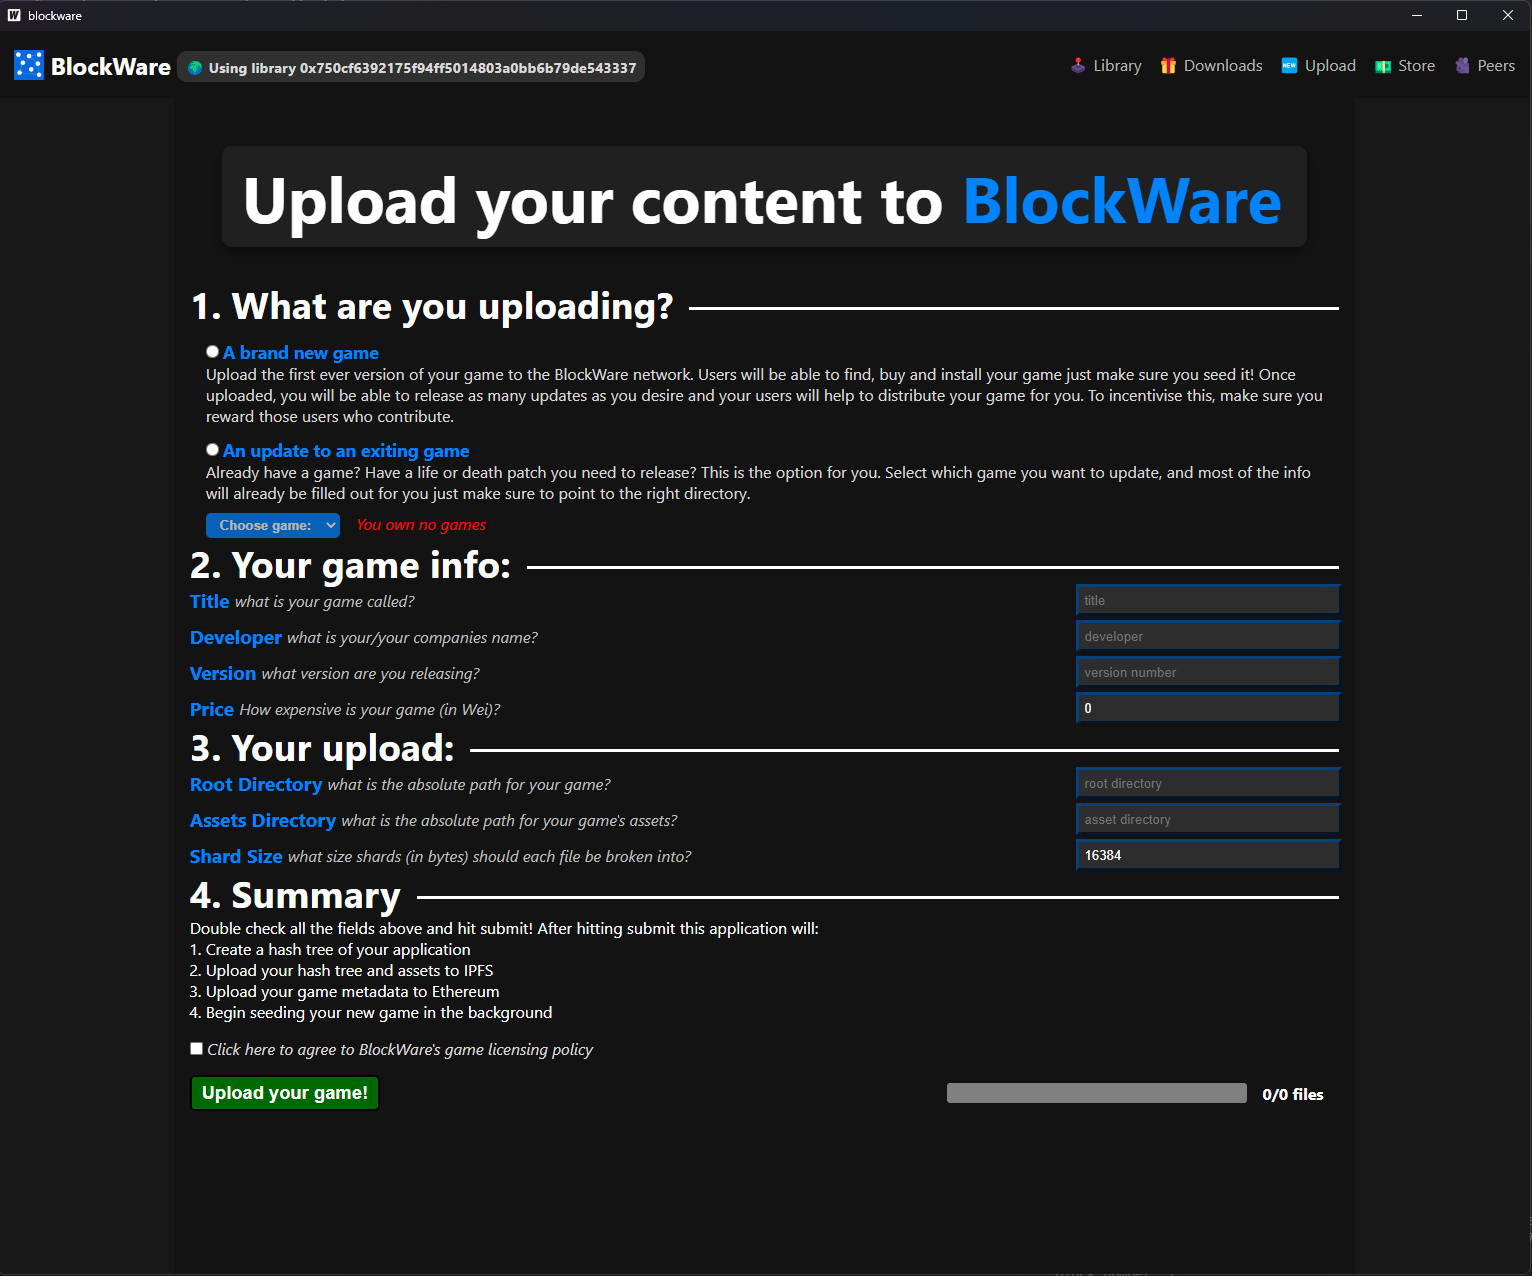
\includegraphics[width=0.9\textwidth]{assets/images/screenshots/upload.png}
  \caption{The page where users input the details about their game and can upload it to the Ethereum network. If a user wants to update a game they can choose from their uploaded games.}
\end{figure}

\begin{figure}[H]
  \centering
  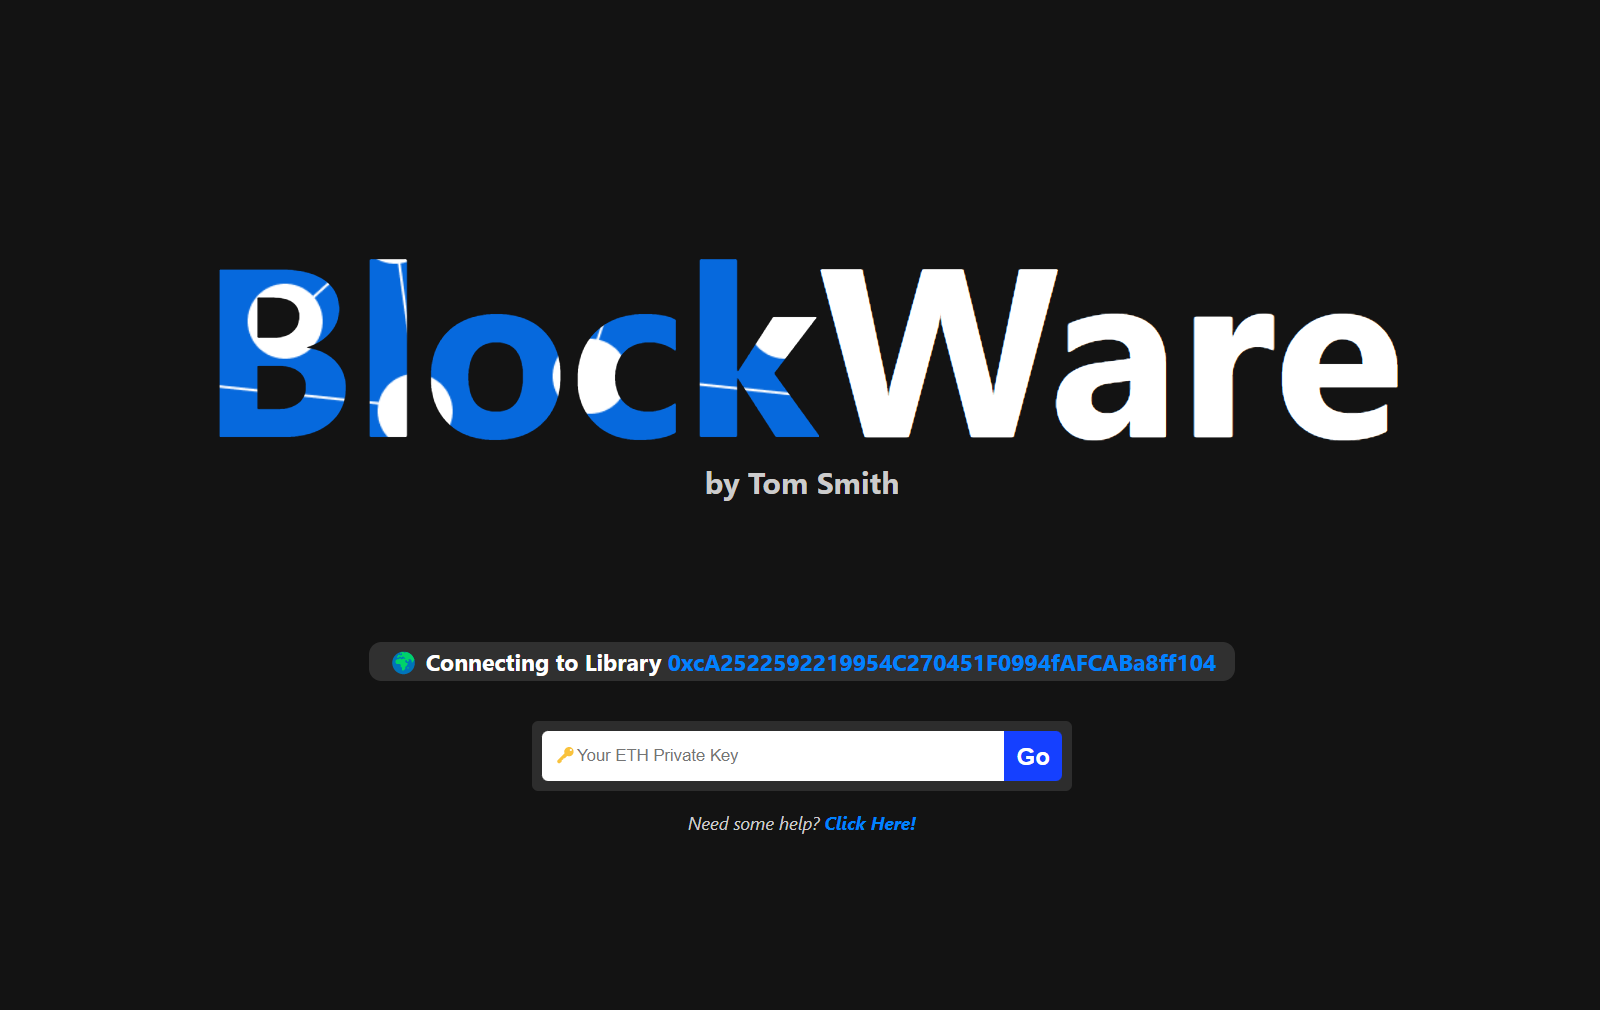
\includegraphics[width=0.9\textwidth]{assets/images/screenshots/login.png}
  \caption{The login page where a user will enter their Ethereum private key and connect to the BlockWare contract instance deployed to Sepolia. Users can access the help page from here.}
\end{figure}

\begin{figure}[H]
  \centering
  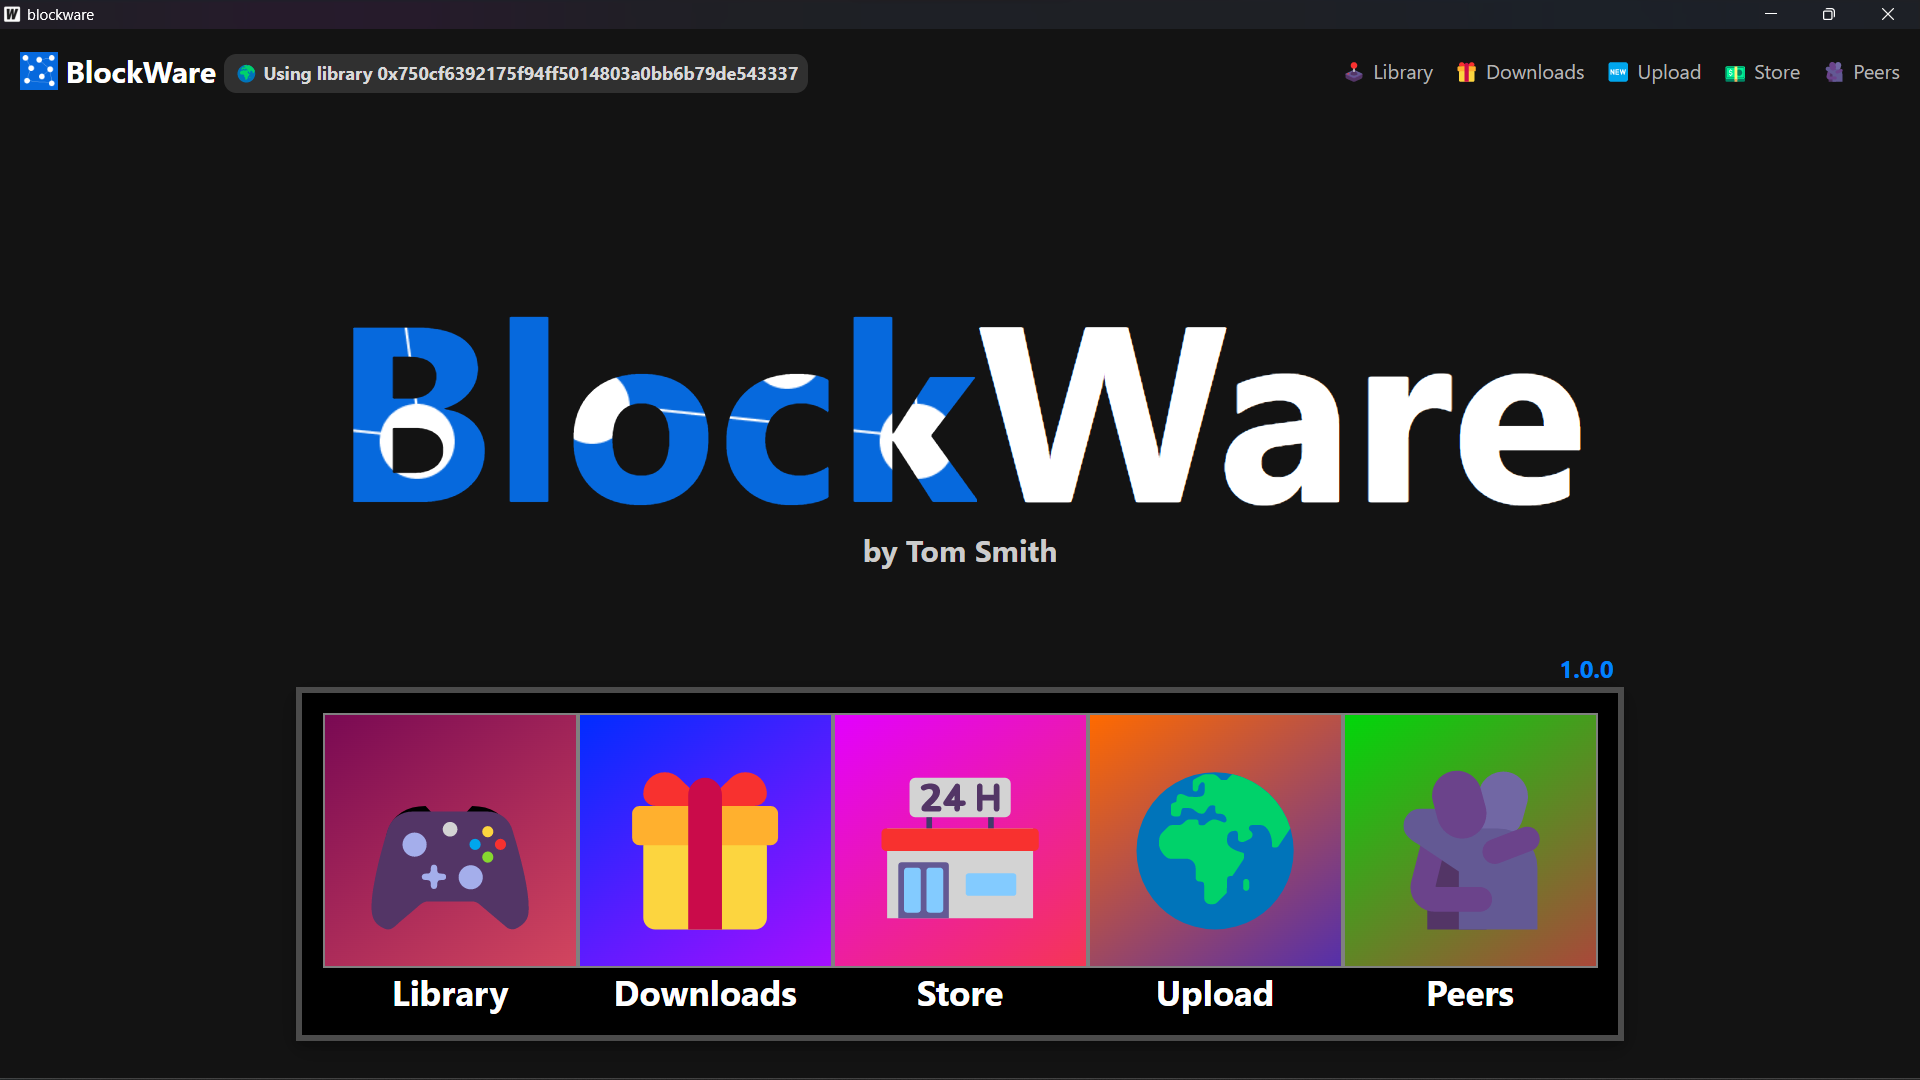
\includegraphics[width=0.9\textwidth]{assets/images/screenshots/home.png}
  \caption{The home page where users can navigate between the main pages.}
\end{figure}

\begin{figure}[H]
  \centering
  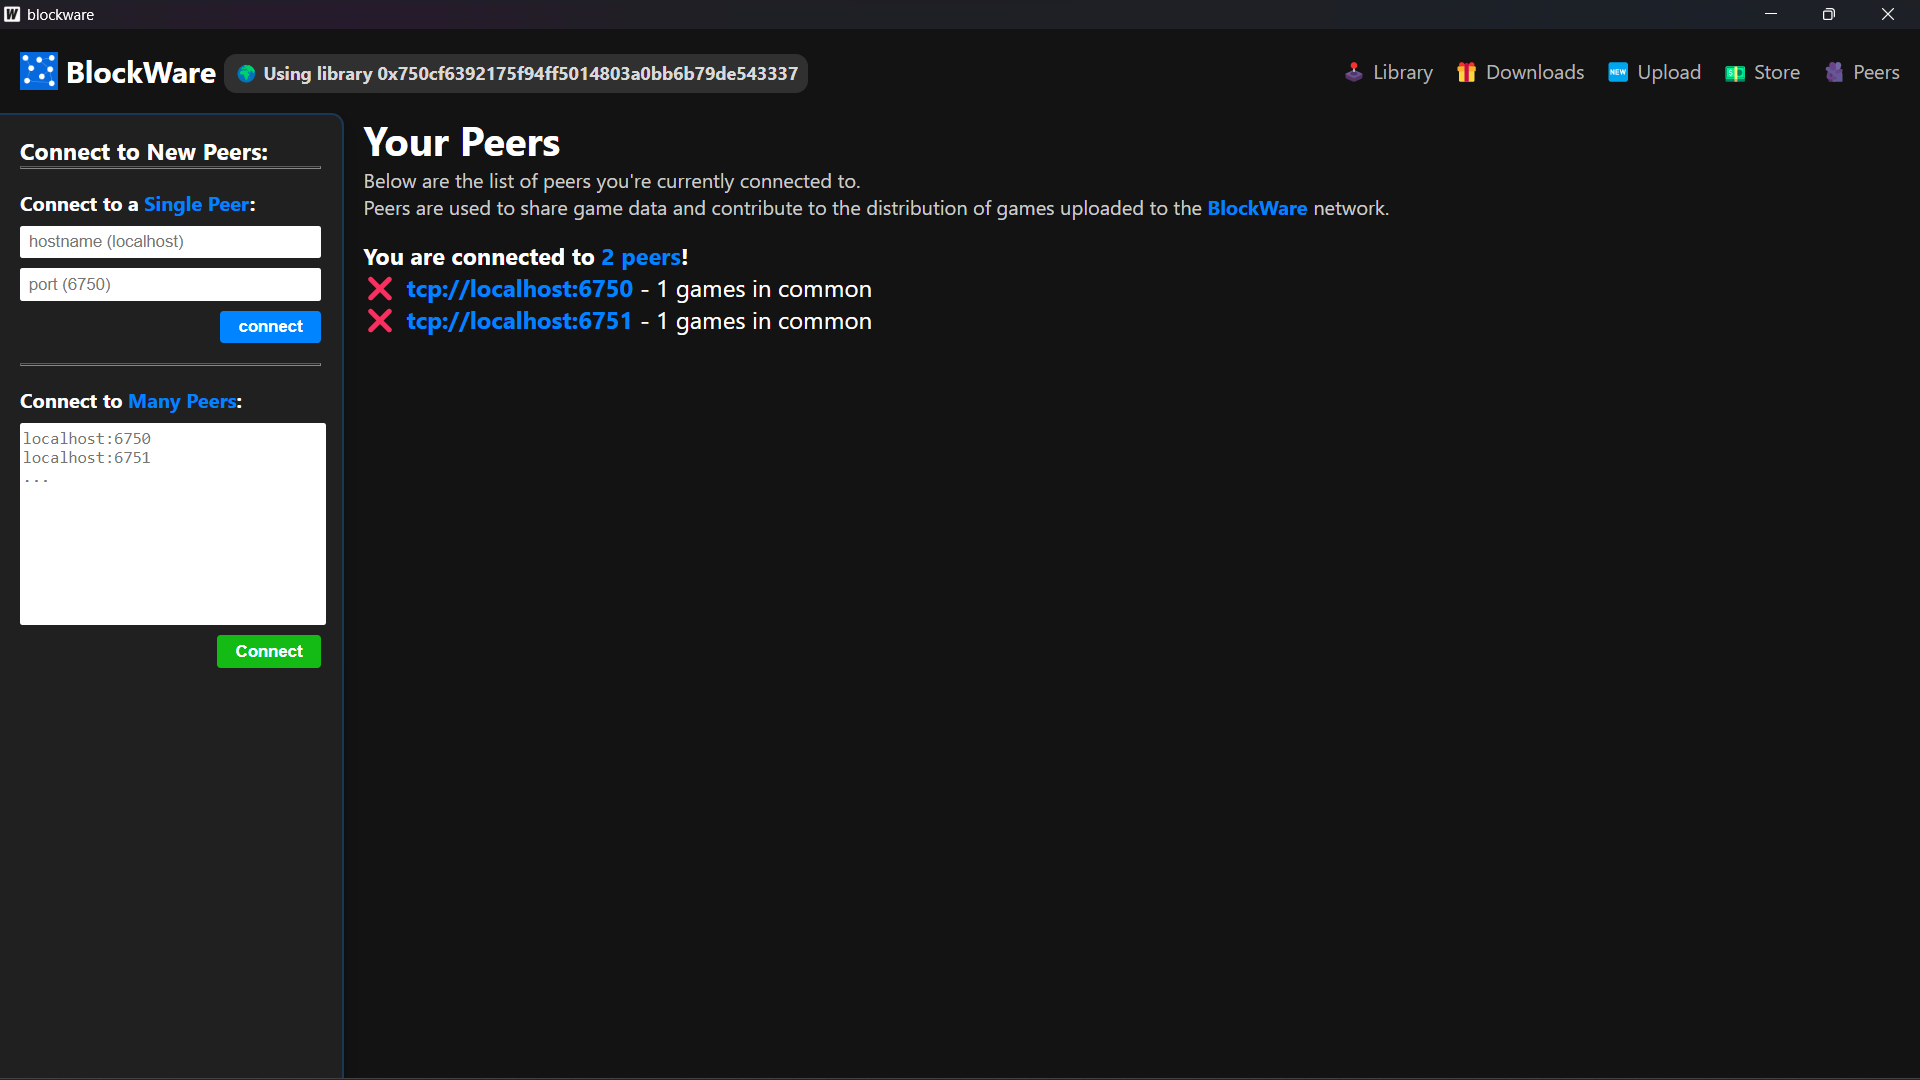
\includegraphics[width=0.9\textwidth]{assets/images/screenshots/peers.png}
  \caption{The page where users can manage their connections to peers with whom they will download game data off of. Users can request receipts from peers that show the amount of data they've sent.}
\end{figure}

\begin{figure}[H]
  \centering
  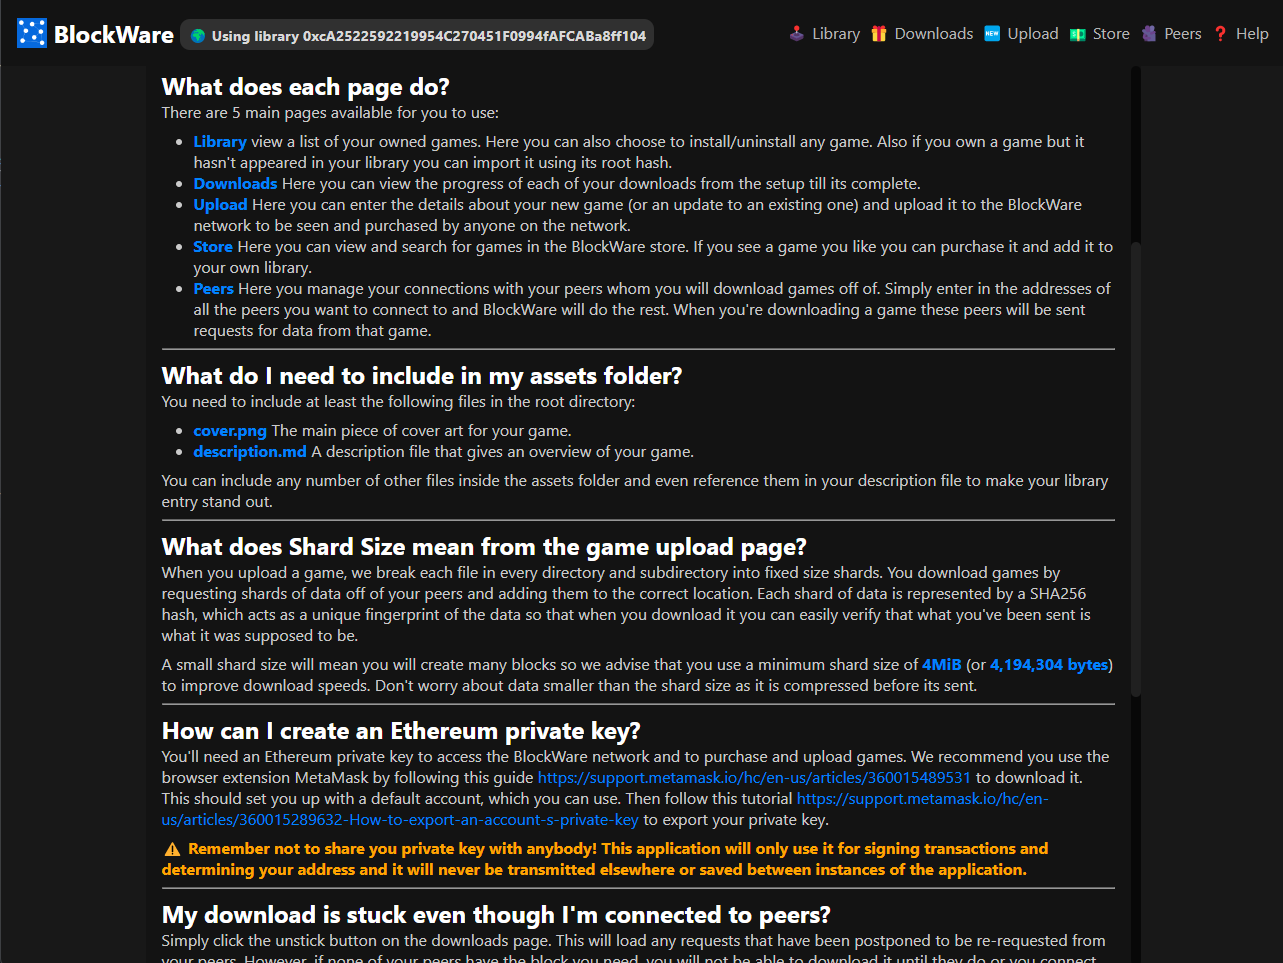
\includegraphics[width=0.9\textwidth]{assets/images/screenshots/help.png}
  \caption{This page has a list of common questions, about the application, expected by users with answers.}
\end{figure}

\begin{figure}[H]
  \centering
  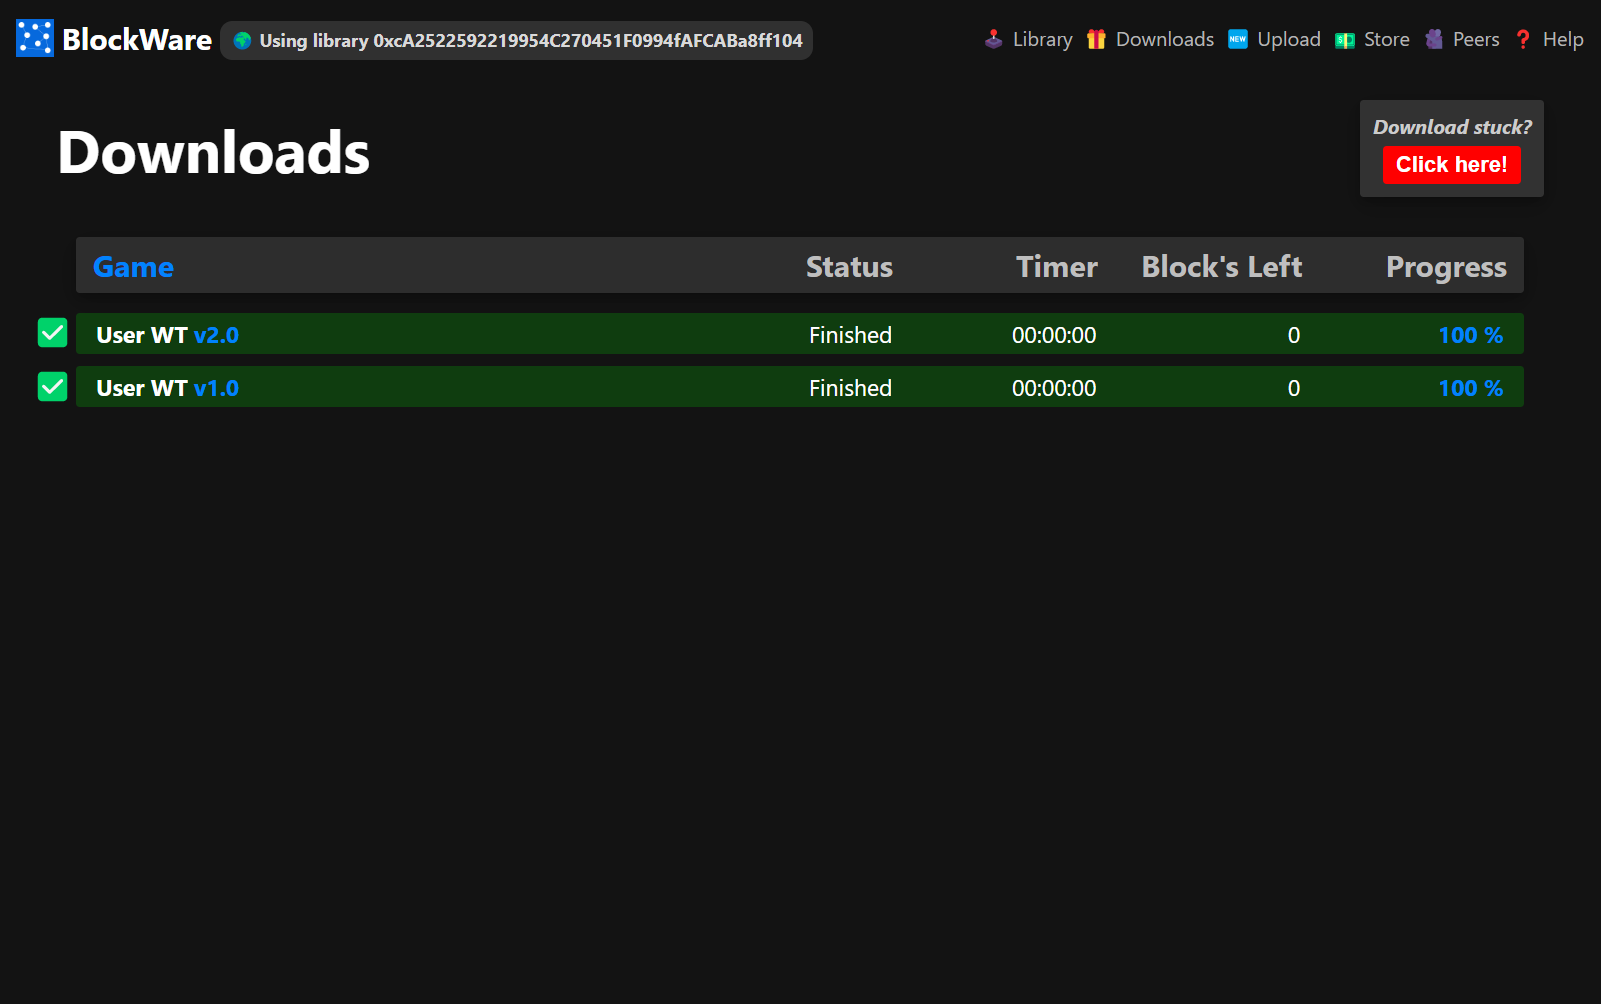
\includegraphics[width=0.9\textwidth]{assets/images/screenshots/downloads.png}
  \caption{This page is where users can track their downloads. It will update in real-time as data is downloaded.}
\end{figure}

\begin{figure}[H]
  \centering
  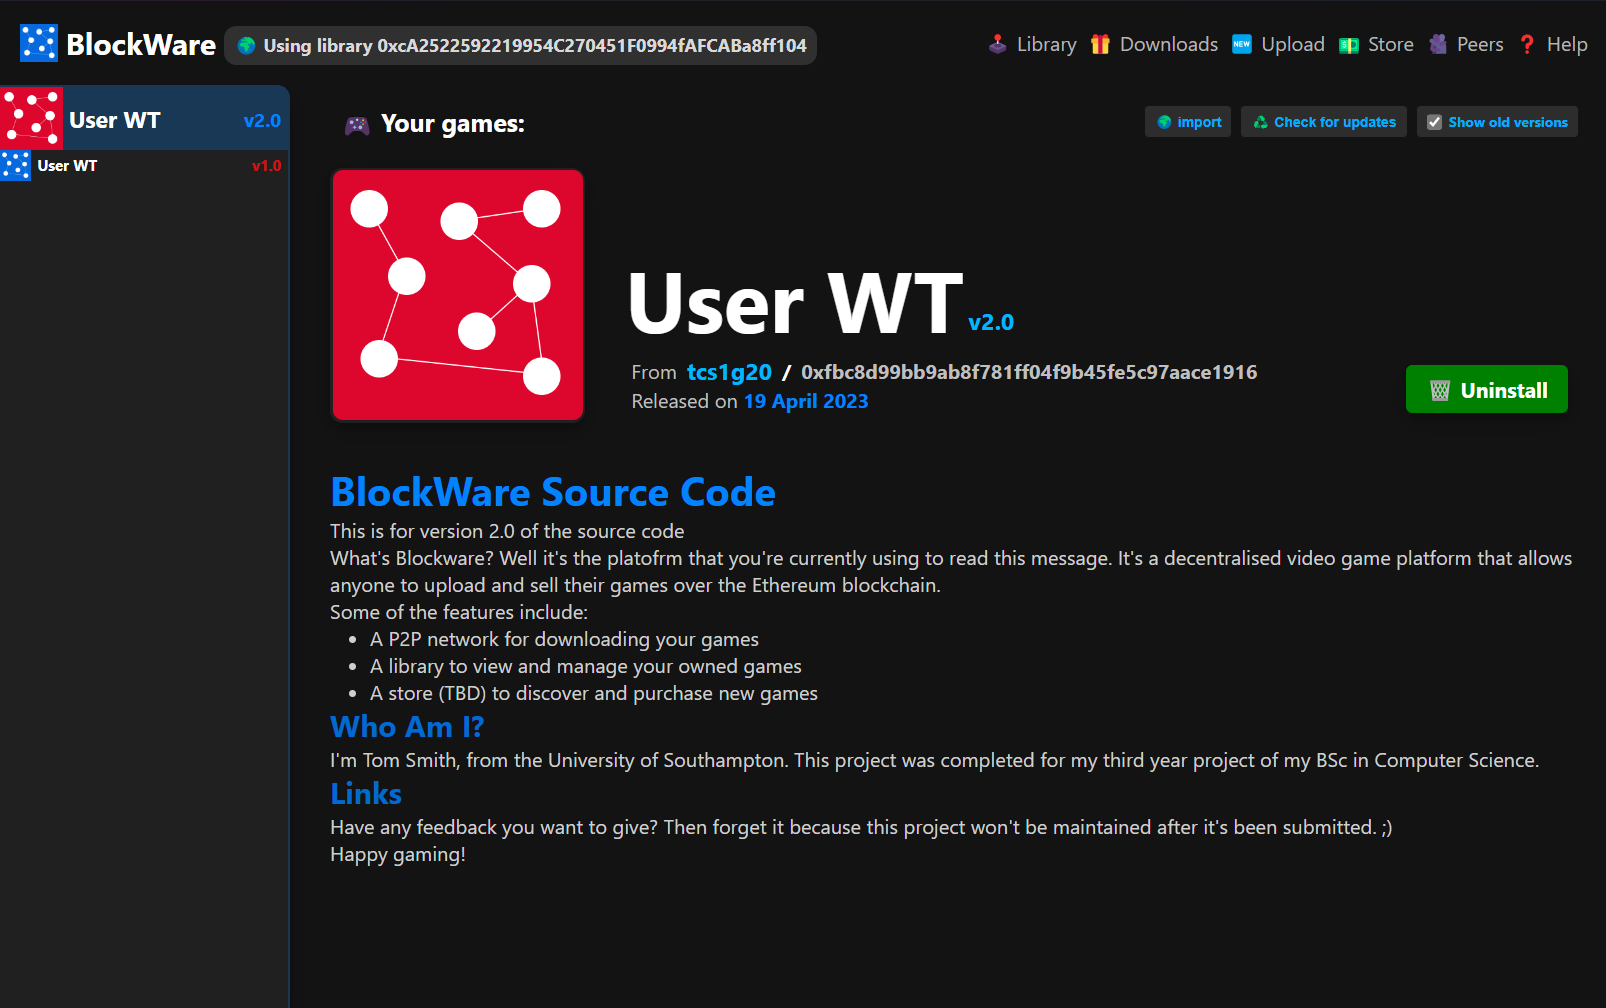
\includegraphics[width=0.9\textwidth]{assets/images/screenshots/library.png}
  \caption{This page shows the user's library of games and allows them to view the assets for them. Smaller games represent older versions of the game and these can be hidden using a the `show old versions' toggle.}
\end{figure}







\chapter{Other Diagrams}

\section*{Requirement Analysis}\label{app:req-analysis}

Figure~\ref{fig:req-generator} shows a mind-map which shows the relationships between primary stakeholders, key pieces of data and key technologies that were expected to be of use for this project. This allowed me to come up with a suitable set of requirements.

\begin{figure}[ht]
  \centering
  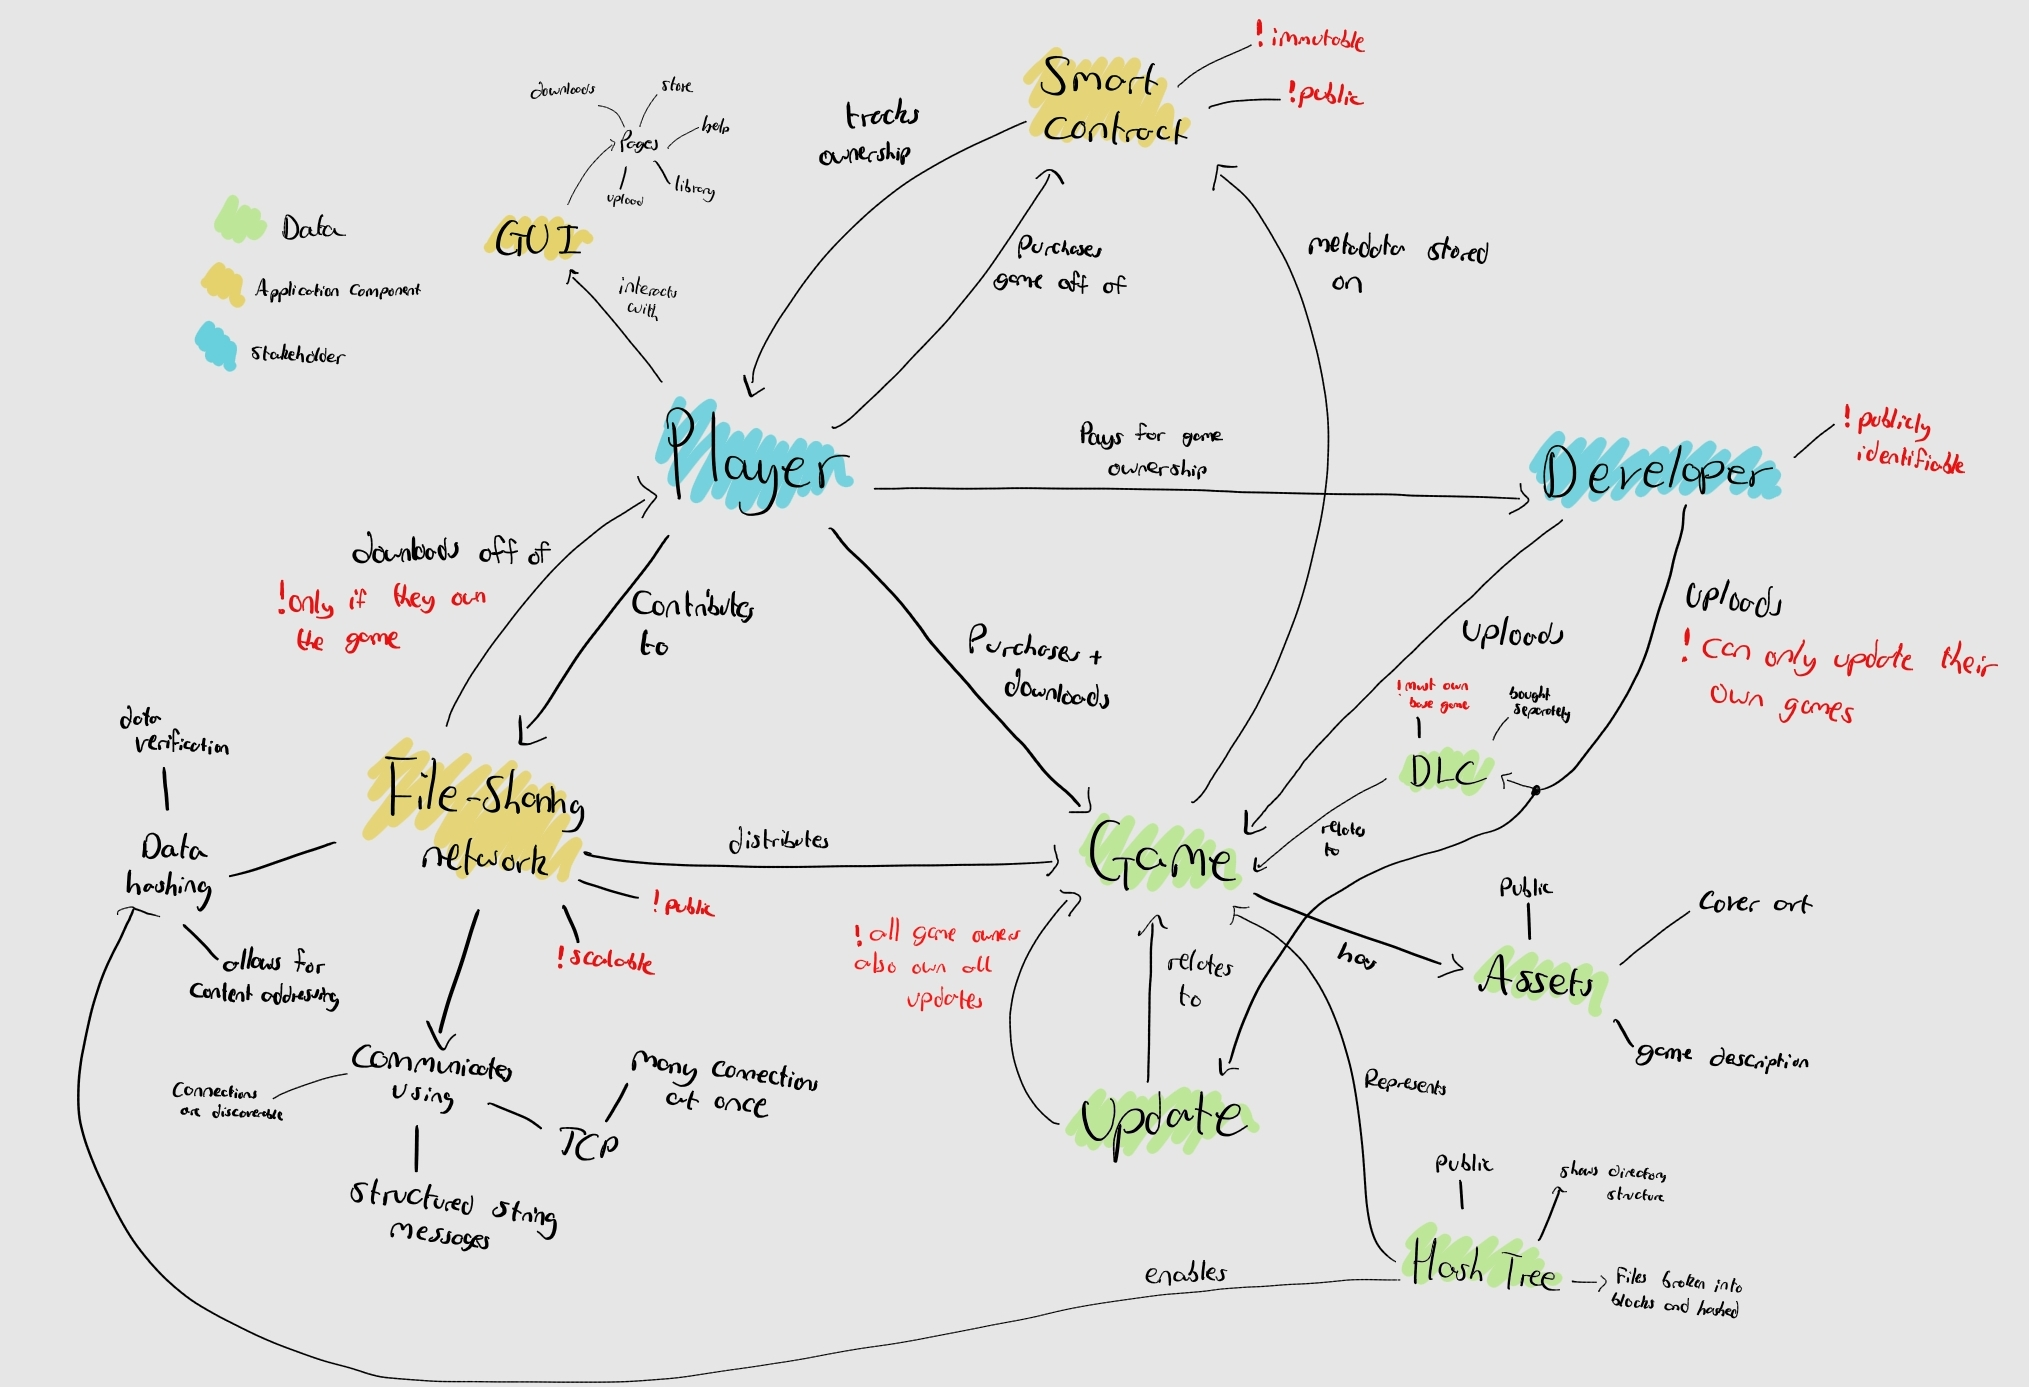
\includegraphics[width=.9\textwidth]{assets/images/diagrams/requirement-generation.jpg}
  \caption{How key elements of the project are related to each other. This diagram was used to help determine the requirements for the application.}
  \label{fig:req-generator}
\end{figure}


\chapter{Progress Report}
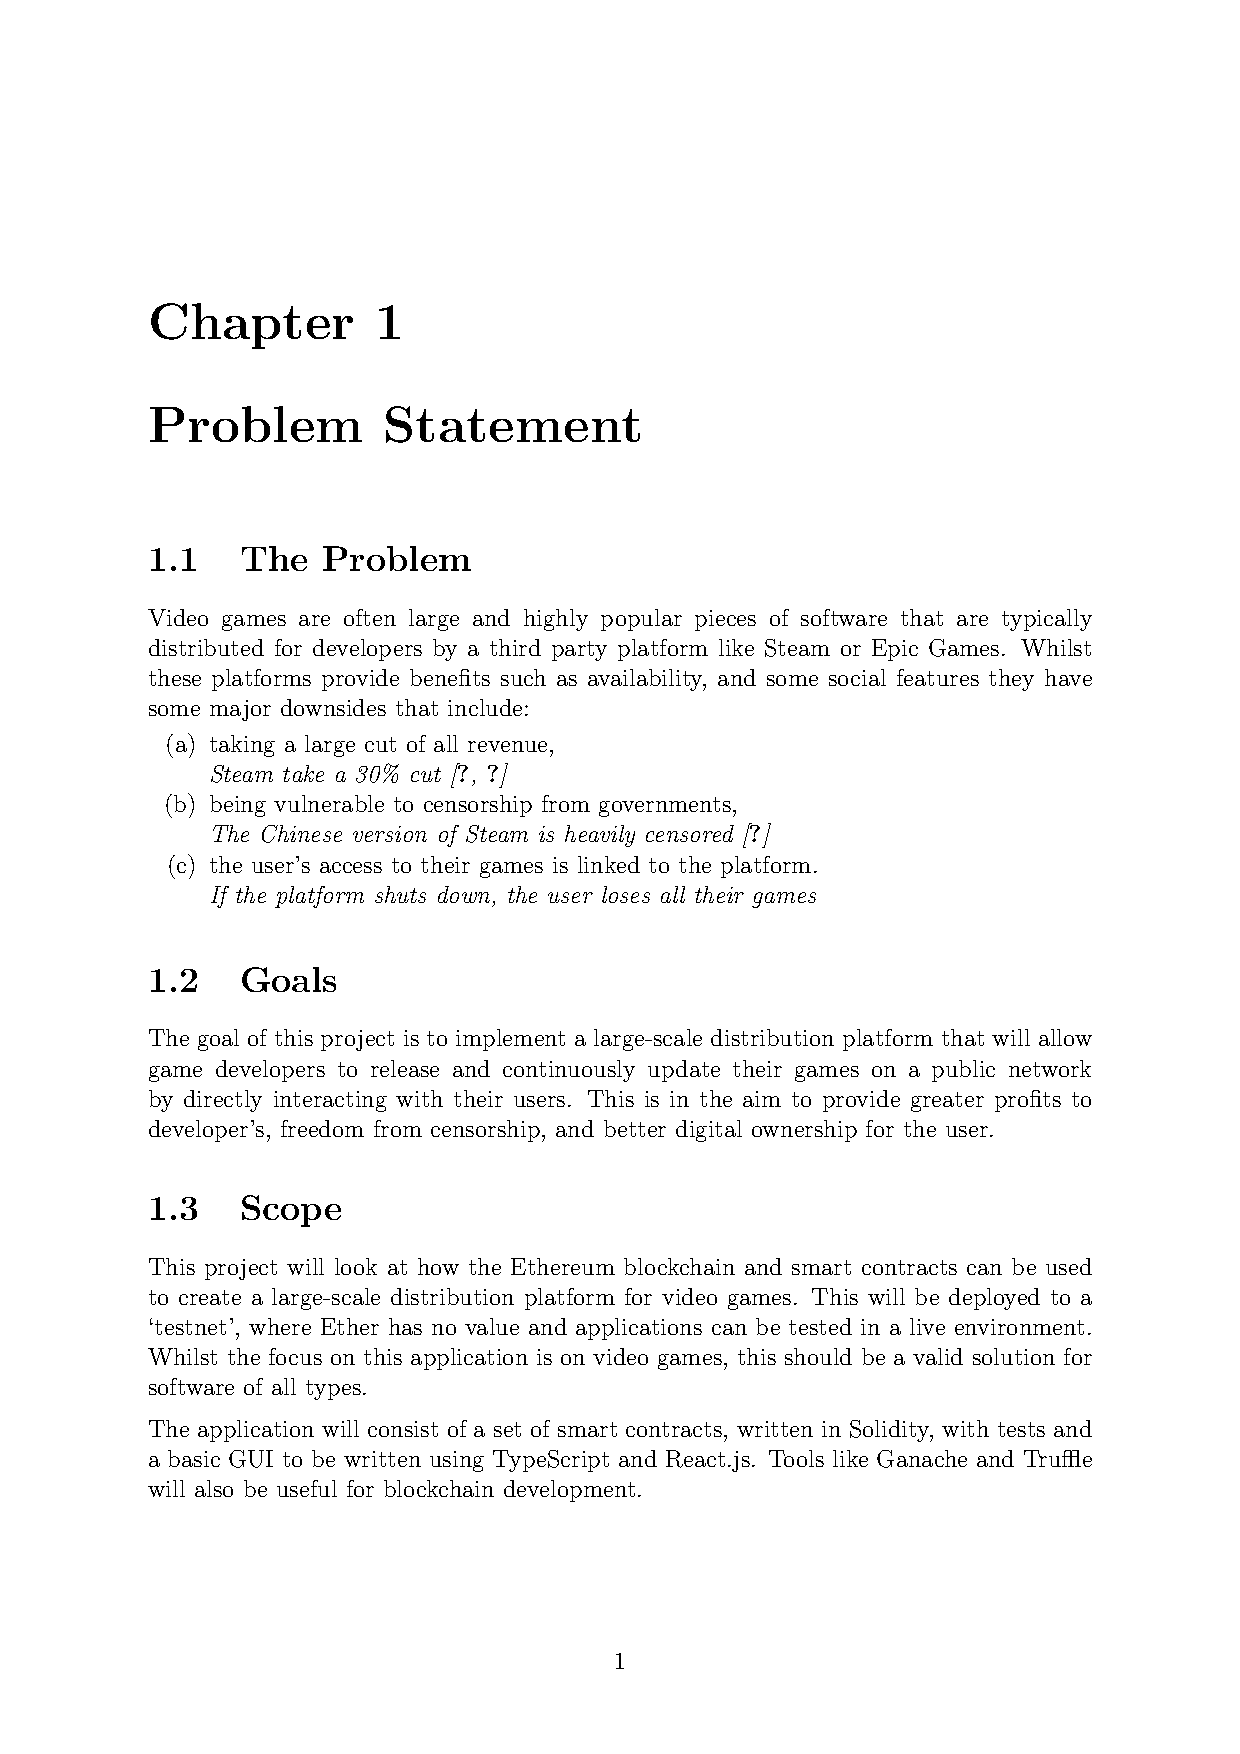
\includepdf[pages=-, pagecommand={\thispagestyle{fancy}}]{assets/InterimBody.pdf}
\fi

\end{document}